%%\iftrue
%\iffalse
%
%\documentclass[12pt, a4paper, oneside]{book}
%% todo: fix appearances
%\usepackage[backend=biber]{biblatex}
%\addbibresource{references.bib}
%
%\usepackage{comment}                            % having comment sections \begin{comment} \end{comment}
%\usepackage[utf8]{inputenc}						% charactere interpretation
%\usepackage{amsmath}							% math package
%\usepackage{amsfonts}							% font package for math symbols
%\usepackage{amssymb}							% symbols package - definition of math symbols
%\usepackage{listings}							% package for code representation
%\usepackage{csquotes}       % Quotation support
%\usepackage{graphicx}							% for inclusion of image
%\setlength {\marginparwidth }{2cm}
%\usepackage{todonotes}
%\usepackage{booktabs}       % Better tables
%\usepackage{caption}        % Better captions
%\usepackage{subfig}								% to arrange figures next to each other
%\usepackage{float}								% text style surrounding images
%\usepackage{threeparttable}
%\usepackage{tikz}								% used to place logos on title page
%% \usepackage{gensymb}							% for special characters such as °
%\usepackage{titlesec}
%\usepackage{multirow}
%\usepackage{siunitx}
%\usepackage{tabularx}
%\usepackage{tikzscale}
%% Format chapter titles without "Chapter X" prefix
%\titleformat{\chapter}[hang]
%{\normalfont\LARGE\bfseries}  % Style: Large bold text
%{\thechapter}                 % Number format: Just the number
%{1em}                         % Space between number and title
%{}                            % Code before the title (empty)
%\usepackage{hyperref}
%\hypersetup{hidelinks}
%\usepackage[acronym]{glossaries}         				% package for glossary
%\makenoidxglossaries
%\newacronym{HSLU}{HSLU}{Lucerne University of Applied Sciences and Arts}
\newacronym[see={[Glossary:]{fitzpatrick-skin-type}}]{FST}{FST}{Fitzpatrick skin type\glsadd{fitzpatrick-skin-type}}
\newacronym{ML}{ML}{Machine Learning}
\newacronym{AI}{AI}{Artificial Intelligence}
\newacronym{FPR}{FPR}{false positive rate}
\newacronym{TPR}{TPR}{true positive rate}
                                % include acronyms.txt file
%\newglossaryentry{fitzpatrick-skin-type}{
	name={Fitzpatrick skin type},
	plural={Fitzpatrick skin types},
	description={A skin classifier based on the skins' reaction to ultraviolet light, developed by dermatologist Dr. Thomas Fitzpatrick \autocite{Gottfrois2024}}
}
\newglossaryentry{JupyterNotebook}{
	name={Jupyter Notebook},
	description={Executable files, often used in ML to write Python code and add explanations in text form}
}
\newglossaryentry{gpuhub}{
	name={GPUhub},
	description={\gls{HSLU}’s server infrastructure for GPU-related computing. It provides isolated environments with JupyterLab access for developing and running \gls{ML} workflows}
}
\newglossaryentry{pediatric}{
	name={pediatric},
	description={A medical term for infants, children and adolescents \autocite{Farlex_nodate}}
}
\newglossaryentry{proxyVar}{
	name={proxy variable},
	plural={proxy variables},
	description={"one or more variables that encode the protected attribute with a substantial degree of accuracy" \autocite{Wang_2021}}
}
\newglossaryentry{teledermatology}{
	name={teledermatology},
	description={dermatological care from a distance, supported by modern technology \autocite{Pala_2020}}
}
\newglossaryentry{Fairlearn}{
	name=Fairlearn,
	description={A Python library for assessing and improving fairness in machine learning models. It supports various fairness metrics and mitigation techniques, especially for binary classification tasks \autocite{Fairlearn_nodate}}
}
\newglossaryentry{Equalized-Odds-Difference}{
	name={equalized odds difference},
	description={The absolute difference in true positive and false positive rates between subgroups, used as a group fairness metric \autocite{Fairlearn_nodate}}
}
\newglossaryentry{Equalized-Odds-Ratio}{
	name={equalized odds ratio},
	description={The ratio of true positive and false positive rates between subgroups, used as a group fairness metric \autocite{Fairlearn_nodate}}
}                                % include glossary.txt file
%\graphicspath{{figures/}}						    % set path of graphics folder
%% mentioned in header
%\newcommand{\tblWidthDescription}{\hsize=0.6\hsize\raggedright}
%\newcommand{\tblWidthContext}{\hsize=0.2\hsize}
%%improved basic functionality
%\newcommand{\bolditalic}[1]{\textbf{\textit{{#1}}}}
%%indicate citations
%% Define a flag to track whether we're inside a raw citation block
%\newif\ifrawcitationactive
%\rawcitationactivefalse % Default: Not inside a raw citation block
%% Define color commands with conditional checking
%\newcommand{\rawcitationstart}{
%	\color{purple}\rawcitationactivetrue
%}
%\newcommand{\rawcitationend}{
%	\color{black}\rawcitationactivefalse
%}
%\newcommand{\rawcitationusedstart}{\color{violet}}
%\newcommand{\rawcitationusedend}{%
%	\ifrawcitationactive
%	\color{purple}  % If inside rawcitation, reset to purple
%	\else
%	\color{black}  % Otherwise, reset to black
%	\fi
%}
%\begin{document}
%\fi
	
	\begin{refsection}
		\chapter{List of Biases}\label{app:listOfBiases}
		The biases are categorized and the relevance for PASSION is added to their chapter title in italic, e.g. \textit{high}.
		
		\section{\textbf{Category:} Sampling Bias}
		Sampling biases occur when the process of collecting data results in samples that are not representative of the broader population. These biases affect the generalisability of machine learning models, especially in medical applications, where population diversity is crucial. According to \textcite{Mehrabi_2021}, non-random or selective sampling can lead to serious consequences in terms of fairness and effectiveness of AI systems.
		
		\subsection{Sampling Bias, \textit{high}}
		\begin{itemize}
			\item \textbf{Definition:} Bias introduced through non-random sampling of subgroups, leading to poor generalisation.
			\item \textbf{Example:} An ML model trained predominantly on patients from urban hospitals may underperform for rural patients.
			\item \textbf{PASSION Relevance:} PASSION aims to address dermatologic sampling bias against highly pigmented skin, but if the included data is not truly representative across populations (e.g., over-representation of certain regions), this could still result in sampling bias \autocite{Mehrabi_2021}.
			\item \textbf{Mitigation Strategy:} Ensure a truly random and inclusive sampling strategy across geography, socioeconomic status, and skin types.
		\end{itemize}
		
		\subsection{Selection Bias, \textit{high}}
		\begin{itemize}
			\item \textbf{Definition:} Bias arising when only a specific subset of the population is used, which is not representative.
			\item \textbf{Example:} Training a model only on adult data, when the target population includes children.
			\item \textbf{PASSION Relevance:} PASSION may suffer from selection bias if only data from severe dermatology cases in hospitals is used \autocites{Mester_2022}{Chakraborty_2024}.
			\item \textbf{Mitigation Strategy:} Include a broad variety of case severities and healthcare settings in the dataset.
		\end{itemize}
		
		\subsection{Systematic Selection Bias, \textit{high}}
		\begin{itemize}
			\item \textbf{Definition:} A form of selection bias where chosen samples differ systematically from the general population.
			\item \textbf{Example:} Including only hospitalized patients in a dataset, while most cases are treated in outpatient settings.
			\item \textbf{PASSION Relevance:} If PASSION uses data only from dermatology centers treating severe cases, it introduces systematic selection bias \autocite{Chakraborty_2024, c5,c6,c33}.
			\item \textbf{Mitigation Strategy:} Include mild, moderate, and severe cases from various clinical settings.
		\end{itemize}
		
		\subsection{Ascertainment Bias, \textit{high}}
		\begin{itemize}
			\item \textbf{Definition:} A systematic distortion arising from the method by which participants or data are selected for inclusion.
			\item \textbf{Example:} Studies on STD prevalence conducted only in public clinics may overlook patients from higher-income backgrounds who go to private practitioners.
			\item \textbf{PASSION Relevance:} If PASSION’s dataset is composed mostly of patients from certain types of clinics, it may not generalise well to other socioeconomic groups \autocite{Chakraborty_2024, c5}.
			\item \textbf{Mitigation Strategy:} Ensure that data is collected from a diverse range of sources, including both public and private healthcare facilities.
		\end{itemize}
		
		\subsection{Availability Bias, \textit{high}}
		\begin{itemize}
			\item \textbf{Definition:} Overreliance on easily accessible data rather than the most representative data.
			\item \textbf{Example:} Using only online available datasets for skin conditions may underrepresent rare diseases.
			\item \textbf{PASSION Relevance:} PASSION inherits availability bias by relying on FST scale–labelled datasets, which may not fully reflect global skin tone diversity \autocites{Chakraborty_2024, c9, c10}.
			\item \textbf{Mitigation Strategy:} Actively seek underrepresented data sources, especially for less common or less documented skin types.
		\end{itemize}
		
		\subsection{Survivorship Bias, \textit{medium}}
		\begin{itemize}
			\item \textbf{Definition:} Only using data from "survivors", i.e., subjects that make it through a certain threshold or are retained in the dataset, ignoring those who were lost earlier.
			\item \textbf{Example:} Evaluating the success of a treatment based only on patients who completed it, ignoring those who dropped out due to side effects.
			\item \textbf{PASSION Relevance:} If certain dermatology diseases are lethal or if the dataset excludes patients unable to attend the centers involved in PASSION, survivorship bias may be present \autocite{Mester_2022}.
			\item \textbf{Mitigation Strategy:} Account for dropout rates and include cases from a wide range of medical access points.
		\end{itemize}
		
		
		\section{\textbf{Category:} Representation Biases}
		Representation biases occur when a sample used to train or evaluate a machine learning model fails to adequately reflect the diversity of the target population. These biases can lead to underperformance for certain subgroups and may negatively impact the fairness and accuracy of a model in real-world applications. In the context of dermatology, these biases could result in skin diseases being underrepresented or misclassified in specific demographic groups, leading to poorer diagnostic outcomes for those populations.
		
		\subsection{Representation Bias, \textit{high}}
		\begin{itemize}
			\item \textbf{Definition:} Representation bias arises when the sample used to train a model does not adequately represent all subgroups of the target population, leading to missing or misrepresented characteristics in the data.
			\item \textbf{Example:} If a skin disease detection model is trained predominantly on skin types I-IV, it may struggle to accurately diagnose conditions in individuals with darker skin tones (FST skin types V-VI).
			\item \textbf{PASSION Relevance:} PASSION attempts to mitigate representation bias by including more FST skin types, but challenges may still exist. The dataset could still lack full representation of all diverse skin conditions and demographic factors, leading to potential misdiagnoses or underperformance for specific subgroups.
			\item \textbf{Mitigation Strategy:} A potential mitigation strategy could involve ensuring a more balanced representation of FST skin types, including rare and diverse skin conditions, and periodically reassessing the dataset to ensure comprehensive inclusion of all skin types across various demographics.
		\end{itemize}
		
		\subsection{Population Bias, \textit{medium}}
		\begin{itemize}
			\item \textbf{Definition:} Population bias occurs when the sample's demographic characteristics (such as age, gender, or ethnicity) do not align with the target population, leading to non-representative data.
			\item \textbf{Example:} If a dataset is predominantly comprised of one ethnic group, a model trained on this data may not generalize well to other ethnic groups, especially if the manifestation of skin diseases varies across ethnicities.
			\item \textbf{PASSION Relevance:} PASSION might be impacted by population bias if it is insufficiently diverse in terms of patient demographics (e.g., ethnicity, age). The dataset needs to ensure that skin diseases are accurately represented across different population groups to avoid skewing results and compromising diagnostic accuracy.
			\item \textbf{Mitigation Strategy:} A mitigation strategy could involve collecting data from diverse populations and ensuring the dataset reflects the target population’s demographic diversity, particularly for ethnicities and age groups that may exhibit different disease manifestations.
		\end{itemize}
		
		\subsection{Aggregation Bias, \textit{high}}
		\begin{itemize}
			\item \textbf{Definition:} Aggregation bias occurs when conclusions drawn from the entire population do not apply to individual subgroups, leading to incorrect or generalized assumptions. This bias arises when significant differences between subgroups (such as gender or ethnicity) are not properly accounted for.
			\item \textbf{Example:} A diagnostic model trained on a heterogeneous dataset might fail to capture how skin diseases manifest differently across genders or ethnic groups, potentially leading to misdiagnosis or unequal treatment recommendations.
			\item \textbf{PASSION Relevance:} Aggregation bias is a significant concern in PASSION, particularly since skin diseases can manifest differently across ethnicities, genders, or genetic backgrounds. The model needs to account for these variations to avoid generalized conclusions that might harm certain subgroups.
			\item \textbf{Mitigation Strategy:} To mitigate aggregation bias, the model should incorporate subgroup-specific data and analysis, ensuring that disease manifestations are correctly accounted for and tailored to different demographic characteristics.
		\end{itemize}
		
		\subsection{Simpson's Paradox, \textit{medium}}
		\begin{itemize}
			\item \textbf{Definition:} Simpson's Paradox is a form of aggregation bias where trends that appear in aggregated data may reverse when the data is disaggregated into subgroups. This paradox can lead to misleading conclusions if not properly addressed.
			\item \textbf{Example:} A dataset may show that skin disease detection is more accurate overall for a specific demographic group, but when the data is broken down by age or skin type, the trend reverses for certain subgroups.
			\item \textbf{PASSION Relevance:} Simpson’s Paradox could be an issue in PASSION if aggregated data from different subgroups results in misleading conclusions. For example, overall accuracy may appear high, but specific skin conditions in certain ethnicities or age groups could have lower accuracy when analyzed separately.
			\item \textbf{Mitigation Strategy:} A mitigation strategy would involve analyzing data at both the aggregated and disaggregated levels, ensuring that subgroup-specific trends are considered to avoid false conclusions or the reversal of apparent associations.
		\end{itemize}
		
		
		
		
		
		\section{\textbf{Category:} Measurement Biases}
		Measurement biases occur when the process of choosing, using, or measuring features leads to inaccurate or misleading results. These biases can emerge from various sources such as mismeasured variables, subconscious expectations of researchers, or inconsistencies in human annotation, and they can significantly affect the reliability of the dataset.
		
		\subsection{Measurement Bias, \textit{high}}
		\begin{itemize}
			\item \textbf{Definition:} Measurement bias occurs when features or variables are inaccurately measured or selected, leading to incorrect interpretations of the outcome.
			\item \textbf{Example:} If a proxy variable, such as country of origin, is used to infer ethnicity or genetic background, it could lead to misinterpretation of the data. For instance, the country of origin may not directly correlate with ethnic background, potentially skewing results in genetic or disease research \autocite{Mehrabi_2021}.
			\item \textbf{PASSION Relevance:} In the context of the PASSION dataset, measurement bias could arise if country of origin is misused as a proxy for ethnicity, which is not directly related to genetic predispositions or skin conditions. This could result in misleading conclusions about skin diseases across different demographic groups, potentially amplifying health disparities.
			\item \textbf{Mitigation Strategy:} To mitigate measurement bias in PASSION, careful consideration should be given to the choice of features used in the dataset. Avoiding proxy variables such as country of origin to infer ethnicity and instead focusing on genetically relevant factors could improve the accuracy of the data and its interpretation.
		\end{itemize}
		
		\subsection{Observer Bias, \textit{medium}}
		\begin{itemize}
			\item \textbf{Definition:} Observer bias occurs when researchers or testers influence the results by projecting their expectations or perceptions onto the data collection process, or when different observers report the same observation differently.
			\item \textbf{Example:} A researcher may subconsciously interpret certain skin disease symptoms differently based on their own expectations or biases, leading to inconsistent data collection or interpretation \autocite{Mester_2022}.
			\item \textbf{PASSION Relevance:} In PASSION, observer bias could affect the consistency and reliability of skin disease annotations. For example, a researcher might influence how they categorize or diagnose certain skin diseases based on their personal biases or experience. This could lead to inaccurate classifications, particularly for diseases that are subjective in appearance.
			\item \textbf{Mitigation Strategy:} To address observer bias in PASSION, standardized training for annotators and a clear, objective set of criteria for diagnosis should be implemented. Additionally, using multiple annotators and cross-checking results can help reduce the impact of individual biases.
		\end{itemize}
		
		\subsection{Annotator Bias, \textit{high}}
		\begin{itemize}
			\item \textbf{Definition:} Annotator bias is a form of observer bias where human annotators are influenced by personal background, expectations, or external factors, which can lead to inconsistent or skewed labeling of data \autocite{Montoya_2025}.
			\item \textbf{Example:} If an annotator is more likely to label a darker skin tone as "severe" or "critical" due to personal or cultural biases, this can introduce inaccuracies in the dataset, which may not be representative of the actual severity of the condition.
			\item \textbf{PASSION Relevance:} In PASSION, annotator bias could particularly affect the labeling of skin tones, which are highly subjective and dependent on individual perception. This bias could lead to inconsistent classifications of skin conditions across different demographic groups, which is critical when assessing dermatological diseases in a diverse population.
			\item \textbf{Mitigation Strategy:} To reduce annotator bias in PASSION, a diverse team of annotators should be trained to recognize and overcome their personal biases. Additionally, the annotation process should be regularly audited to ensure consistency, and the use of automated tools for initial labeling could provide more objectivity in the process.
		\end{itemize}
		
		\subsection{Recall Bias, \textit{medium}}
		\begin{itemize}
			\item \textbf{Definition:} Recall bias occurs when individuals do not accurately remember or report information due to selective memory, which can lead to misinterpretations or inaccurate conclusions in data analysis \autocites{Mester_2022}{Chakraborty_2024}.
			\item \textbf{Example:} If patients are asked to recall past skin conditions or treatments, they may forget important details, leading to inaccurate reporting in the dataset. This could affect the analysis of how different skin diseases develop or respond to treatments.
			\item \textbf{PASSION Relevance:} Recall bias may not be directly relevant in the context of PASSION since the dataset appears to rely on clinical observations and annotations rather than patient-reported data. However, if there is any patient input, such as in follow-up surveys or self-reported symptoms, recall bias could still influence the dataset.
			\item \textbf{Mitigation Strategy:} To mitigate recall bias, it would be important to gather more objective data through clinical observations or imaging, and ensure that patient self-reports are validated through corroborating medical records or consistent follow-ups.
		\end{itemize}
		
		\subparagraph{Potential Biases in PASSION}
		Measurement Bias: Country of origin should not be used as a proxy for ethnicity in the PASSION dataset, as it may not be directly related to genetic or disease factors. Additionally, annotator bias regarding skin tone labeling has been investigated in recent studies and should be addressed in PASSION's annotation process \autocite{Montoya_2025}.
		
		
		\section{\textbf{Category:} Research Biases}
		Research biases refer to the ways in which researchers' decisions, intentions, and contexts influence the outcomes of their studies, potentially introducing systematic errors that may affect the validity or generalizability of the findings.
		
		\subsection{Funding / Sponsorship bias, \textit{medium}}
		\begin{itemize}
			\item \textbf{Definition:} Funding or sponsorship bias occurs when research findings are consciously or unconsciously influenced by the expectations or interests of the study’s financial backers. This can lead to findings that favor the sponsor’s interests.
			\item \textbf{Example:} A dermatology study funded by a pharmaceutical company that produces skin disease treatment medications may emphasize the effectiveness of the company's products, even if there is no strong evidence supporting their superiority.
			\item \textbf{PASSION Relevance:} Funding bias could affect the PASSION dataset if the research or data collection process were influenced by sponsors or stakeholders with vested interests in certain outcomes. While this bias is not explicitly mentioned in PASSION, it is important for future studies to ensure that funding sources do not shape data interpretation or collection in a way that would lead to skewed or misleading results.
			\item \textbf{Mitigation Strategy:} To mitigate this, independent funding sources or transparent funding disclosure practices should be implemented. Additionally, external audits or independent validation of the findings can help prevent undue influence from sponsors.
		\end{itemize}
		
		\subsection{Data dredging bias, \textit{low}}
		\begin{itemize}
			\item \textbf{Definition:} Data dredging bias arises when researchers deliberately select statistical methods or models that lead to specific p-values or results, potentially making their hypothesis appear more likely to be true than it actually is.
			\item \textbf{Example:} A researcher testing multiple variables in a dataset might select those combinations that yield the most statistically significant results, even if the relationships between the variables were not hypothesized initially.
			\item \textbf{PASSION Relevance:} Given that PASSION is a large dermatology dataset, it could be vulnerable to data dredging if analysts test many variables or relationships without pre-specified hypotheses. This could lead to spurious findings or models that do not generalize well to new data.
			\item \textbf{Mitigation Strategy:} To avoid data dredging, a clear and well-defined hypothesis should be established before conducting any statistical tests. Additionally, cross-validation techniques and reporting of all tested models can ensure transparency in the research process.
		\end{itemize}
		
		\subsection{Hypothetical bias, \textit{not applicable}}
		\begin{itemize}
			\item \textbf{Definition:} Hypothetical bias occurs when responses to hypothetical questions do not reflect real-world behavior or preferences.
			\item \textbf{Example:} Asking participants how likely they would be to adopt a particular skincare treatment, without actually testing their behavior in real-world settings.
			\item \textbf{PASSION Relevance:} This bias is not applicable to the PASSION dataset, as the dataset does not involve hypothetical scenarios or self-reported intentions. The dataset primarily contains real-world medical data related to dermatology, which does not rely on participant speculation or hypothetical responses.
			\item \textbf{Mitigation Strategy:} Since this bias is not relevant to PASSION, no specific mitigation strategy is necessary.
		\end{itemize}
		
		\paragraph{Potential Biases in PASSION}
		Since the PASSION dataset is already published, the research biases might already be introduced. It is not feasible during the duration of this thesis to make an evaluation on those biases. Instead, I would recommend the PASSION team and researchers in general to check the list above carefully and take measures against them. Maybe, an external evaluation could help to detect and prevent those biases even better.
		
		
		\section{\textbf{Category:} Feature Representation Biases}
		Feature representation biases occur when the features or variables used in a model do not adequately capture the complexity of the problem or reflect all relevant aspects of the data, potentially leading to biased or incomplete predictions.
		
		\subsection{Omitted Variable Bias, \textit{high}}
		\begin{itemize}
			\item \textbf{Definition:} Omitted variable bias arises when key variables are left out of a model, causing the model to be unprepared to account for certain aspects of the data and potentially leading to biased or inaccurate predictions.
			\item \textbf{Example:} If a dermatology model only includes skin condition data but omits important demographic information such as ethnicity or age, it may fail to identify or misinterpret certain patterns in the data.
			\item \textbf{PASSION Relevance:} The PASSION dataset has an omission of ethnicity as a feature, which could lead to biased results. Certain skin diseases and their manifestation can vary significantly across different ethnic groups. Without this variable, the model may fail to capture important differences in the data, leading to inaccurate predictions or generalizations.
			\item \textbf{Mitigation Strategy:} To address this bias, it is important to include a comprehensive set of features, such as ethnicity, age, gender, and other demographic factors, which could help the model better account for variations in skin conditions across different populations.
		\end{itemize}
		
		\subsection{Collider Bias, \textit{medium}}
		\begin{itemize}
			\item \textbf{Definition:} Collider bias occurs when two variables influence a common third variable (the collider variable), and the analysis restricts sampling based on this collider, leading to a distorted or biased relationship between the variables.
			\item \textbf{Example:} In the case of skin disease models, if researchers only include patients who seek treatment for a specific skin condition (the collider), this may limit the analysis to a non-representative sample, potentially distorting the relationship between disease characteristics and other factors.
			\item \textbf{PASSION Relevance:} Although no specific collider bias has been identified in PASSION, it is important to consider that factors like patient willingness to seek treatment or the specific type of skin disease could act as collider variables. Restricting the dataset based on these factors might create a biased representation of the population.
			\item \textbf{Mitigation Strategy:} To reduce collider bias, it is important to ensure that the sample is as representative as possible of the broader population. Researchers should avoid restrictions that could inadvertently create a non-representative dataset and be mindful of how their sampling methods may introduce bias.
		\end{itemize}
		
		\subparagraph{Potential Biases in PASSION}
		The PASSION dataset may suffer from omitted variable bias, particularly with the lack of ethnicity data, which can affect the fairness and accuracy of dermatology models. Collider bias could also emerge depending on how the dataset is sampled or restricted based on treatment-seeking behavior or disease severity. It is important for researchers to monitor for these biases and take steps to mitigate them by ensuring that data collection and sampling strategies are inclusive and comprehensive.
		
		
		
		\section{\textbf{Category:} Imaging Biases}
		Imaging biases refer to the influence that technical variations, environmental factors, and other visual elements have on image-based classification systems. These biases can arise from issues such as the quality of the image, artifacts present in the image, or the field of view captured, which can all influence the performance of machine learning models.
		
		\subsection{Image Quality Bias, \textit{high}}
		\begin{itemize}
			\item \textbf{Definition:} Image quality bias occurs when the quality of an image—such as the zoom level, focus, or lighting—affects how a machine learning model classifies or diagnoses the image. Poor image quality can lead to misclassification or lower prediction accuracy.
			\item \textbf{Example:} If a dermatologist captures an image with insufficient lighting or poor focus, the model may struggle to identify skin conditions like melanomas, potentially leading to a misdiagnosis.
			\item \textbf{PASSION Relevance:} In the PASSION dataset, variations in image quality could lead to biased predictions. For instance, images captured under different lighting conditions or at varying zoom levels might cause the model to overfit to certain image qualities, mistaking them for certain conditions. This could reduce the model’s generalizability to diverse real-world conditions.
			\item \textbf{Mitigation Strategy:} To mitigate image quality bias, it is essential to standardize image acquisition protocols and pre-process images to normalize variations in quality. Implementing techniques like image enhancement and quality control during data collection could help improve model performance.
		\end{itemize}
		
		\subsection{Visual Artifact Bias, \textit{high}}
		\begin{itemize}
			\item \textbf{Definition:} Visual artifact bias arises from artifacts in dermatology images, such as hair, surgical ink markings, or other extraneous elements that could interfere with accurate classification of skin diseases.
			\item \textbf{Example:} A photograph of a skin lesion may contain hair or tattoos from previous medical procedures, making it more difficult for the model to identify the skin condition correctly.
			\item \textbf{PASSION Relevance:} The PASSION dataset may include dermatology images with artifacts like surgical markings or hair, which could confuse the model into associating these artifacts with the presence of a skin disease. This could lead to incorrect predictions, especially if the model cannot differentiate between the artifact and the actual lesion.
			\item \textbf{Mitigation Strategy:} To reduce visual artifact bias, it is important to implement preprocessing steps that remove or mask artifacts in images. This could involve techniques such as hair removal or the use of clean, artifact-free image samples for training.
		\end{itemize}
		
		\subsection{Field of View Bias, \textit{high}}
		\begin{itemize}
			\item \textbf{Definition:} Field of view bias occurs when the portion of the body or skin that is captured in an image is limited, affecting how well a model can classify a skin condition. Different angles, distances, or body parts in the view may lead to different prediction results.
			\item \textbf{Example:} If only a small portion of a skin lesion is captured in the image (e.g., just the edge of a mole), the model may miss critical features needed to correctly identify melanoma or other conditions.
			\item \textbf{PASSION Relevance:} In the PASSION dataset, field of view bias could emerge if certain lesions are captured from angles or in parts of the body that limit the information available for accurate classification. This could result in the model underperforming on images that are not representative of common views of skin conditions.
			\item \textbf{Mitigation Strategy:} To address field of view bias, the dataset should ensure that images are captured from standardized and consistent angles or distances. Augmenting the dataset with a variety of views from multiple angles could help improve the model's ability to generalize to unseen cases.
		\end{itemize}
		
		\subparagraph{Potential Biases in PASSION}
		The PASSION model could learn to associate unrelated visual effects, hair, body parts, or image quality with a disease, which could impact its performance. Ensuring standardized image acquisition methods and removing artifacts could mitigate some of these biases.
		
		\section{\textbf{Category:} Medical Biases}
		Medical biases are specific to healthcare-related machine learning applications and can have direct implications for diagnosis, treatment, and patient outcomes. These biases often arise from the healthcare system’s structure and can lead to distorted or inaccurate predictions based on incomplete or unrepresentative data.
		
		\subsection{Berkesonian Bias, \textit{medium}}
		\begin{itemize}
			\item \textbf{Definition:} Berkesonian bias occurs in hospital-based studies when certain factors (such as disease severity or risk factors) influence whether patients seek treatment or are hospitalized. This can distort the relationship between variables due to the study population being unrepresentative of the general population.
			\item \textbf{Example:} In a study focusing on skin diseases, if only patients who sought care for severe conditions are included, the relationship between disease severity and other factors could be overstated, leading to inaccurate conclusions.
			\item \textbf{PASSION Relevance:} The PASSION dataset could be influenced by Berkesonian bias if the images are sourced only from patients who visited certain hospitals or dermatologists, potentially skewing the representation of less severe or untreated conditions. This could limit the model's generalization to populations with different healthcare access.
			\item \textbf{Mitigation Strategy:} To mitigate Berkesonian bias, it is important to include a diverse set of patients from multiple sources, including both hospital and non-hospital populations, ensuring a more representative dataset.
		\end{itemize}
		
		\subsection{Informed Presence Bias, \textit{medium}}
		\begin{itemize}
			\item \textbf{Definition:} Informed presence bias occurs when individuals who seek medical care are more likely to be screened for other diseases. This bias can result in misleading interpretations of the relationships between diseases.
			\item \textbf{Example:} A person who is already being treated for one skin condition might also be screened for other conditions, leading to a misinterpretation of comorbidities or a false relationship between conditions.
			\item \textbf{PASSION Relevance:} In the PASSION context, informed presence bias could affect correlations between different skin diseases. If patients with certain conditions are more likely to seek treatment, the model might overestimate the likelihood of co-occurrence between those conditions.
			\item \textbf{Mitigation Strategy:} To reduce informed presence bias, the model should account for patients with varying levels of care-seeking behavior and ensure that both treated and untreated conditions are represented in the dataset.
		\end{itemize}
		
		\subsection{Diagnostic Access Bias, \textit{medium}}
		\begin{itemize}
			\item \textbf{Definition:} Diagnostic access bias occurs when individuals in certain geographical locations have better access to medical care, leading to earlier diagnosis and potentially higher disease prevalence in those regions.
			\item \textbf{Example:} Patients in urban areas with better healthcare access may receive earlier diagnoses of skin conditions like melanoma, while those in rural or underserved areas may have their conditions diagnosed at a later stage.
			\item \textbf{PASSION Relevance:} PASSION attempts to address diagnostic access bias by including samples from later stages of diseases. However, it could still be relevant if the dataset over-represents well-diagnosed cases from areas with better healthcare access, skewing the distribution of disease stages.
			\item \textbf{Mitigation Strategy:} To address diagnostic access bias, it is important to ensure that the dataset includes a diverse range of geographical locations and healthcare access levels, including both early and late-stage conditions.
		\end{itemize}
		
		\subsection{Diagnostic Reference Test Bias, \textit{medium}}
		\begin{itemize}
			\item \textbf{Definition:} Diagnostic reference test bias occurs when not all individuals in a study receive the same reference test, leading to discrepancies in diagnoses.
			\item \textbf{Example:} Inconsistent use of reference tests across different hospitals or dermatologists may result in different diagnoses for the same patient, causing confusion and inconsistency in the results.
			\item \textbf{PASSION Relevance:} Depending on how dermatologists work in the PASSION dataset, diagnostic reference test bias could be present. If different diagnostic methods or reference tests are used, the model may learn to associate certain diagnostic practices with specific diseases, rather than the diseases themselves.
			\item \textbf{Mitigation Strategy:} To mitigate diagnostic reference test bias, it is important to standardize the diagnostic processes across different healthcare settings and ensure consistent use of reference tests when collecting data.
		\end{itemize}
		
		\subparagraph{Potential Biases in PASSION}
		Some of the medical biases that could impact PASSION include Berkesonian bias, informed presence bias, diagnostic access bias, and diagnostic reference test bias. Each of these could influence how the model generalizes to real-world populations. Addressing these biases requires careful consideration of the dataset’s diversity and the standardization of diagnostic practices across different settings.
		
		
		\section{\textbf{Category:} Temporal Biases}
		Temporal biases arise due to differences in populations and their behavior over time. These biases can manifest when studying the progression of diseases or tracking changes in populations over time. In studies where data are collected over extended periods, temporal biases can affect the accuracy and generalizability of the results.
		
		\subsection{Longitudinal Data Fallacy, \textit{not applicable}}
		\begin{itemize}
			\item \textbf{Definition:} Longitudinal data fallacy refers to the misinterpretation or improper use of data collected over time, often caused by overlooking important variables or assuming temporal relationships without proper evidence.
			\item \textbf{Example:} A study might incorrectly assume that a disease progression observed over a period directly results from the treatment being applied, while other confounding factors may also play a role.
			\item \textbf{PASSION Relevance:} Temporal biases such as longitudinal data fallacy do not apply to the PASSION dataset, as it does not track disease progression over time but instead consists of static images that are not connected to temporal data.
			\item \textbf{Mitigation Strategy:} Since the PASSION dataset does not involve longitudinal data, no mitigation strategy is necessary for this particular bias.
		\end{itemize}
		\subsection{Chronological Bias, \textit{not applicable}}
		\begin{itemize}
			\item \textbf{Definition:} Chronological bias occurs when the timing of data collection influences the results or introduces errors, often due to the use of data collected at different time points that may not be representative of the population or phenomenon being studied.
			\item \textbf{Example:} If a medical dataset includes only images collected from patients in a certain time period where a specific treatment was more commonly used, the findings might be skewed to reflect outcomes that are not generalizable to other time periods.
			\item \textbf{PASSION Relevance:} Chronological bias is irrelevant to the PASSION dataset as it consists of static images of skin diseases, without any temporal association or tracking of disease progression.
			\item \textbf{Mitigation Strategy:} Since PASSION does not contain temporal data, no mitigation strategy is needed for chronological bias in this case.
		\end{itemize}
		\subsection{Immortal Time Bias, \textit{not applicable}}
		\begin{itemize}
			\item \textbf{Definition:} Immortal time bias refers to a situation where the period of time during which an event could have occurred is misclassified, leading to incorrect conclusions, typically when patients are erroneously considered "at risk" for an event for a period in which the event could not have occurred.
			\item \textbf{Example:} A study that tracks patients who have received a specific treatment might misclassify the time between treatment and disease progression as time "at risk," even though the patients were not at risk during the follow-up period.
			\item \textbf{PASSION Relevance:} Immortal time bias does not apply to PASSION, as the dataset does not track time or disease progression and focuses on static images of skin diseases, eliminating the possibility of immortal time bias.
			\item \textbf{Mitigation Strategy:} No mitigation strategy is necessary for immortal time bias in PASSION, as it is not a relevant concern for the dataset.
		\end{itemize}
		
		\section{\textbf{Category:} Algorithmic Biases}
		When an algorithm adds biases to unbiased input data, it is referred to as \textbf{Algorithmic Bias} \autocite{M9_Baeza-Yates_2018}. This can arise due to various algorithmic design choices such as optimization functions, regularizations, and statistically biased estimators \autocite{M44_Danks_2017}.
		
		\subsection{User Algorithm Interaction Biases, \textit{high}}
		\begin{itemize}
			\item \textbf{Definition:} User interaction biases arise when the user interface or user behavior influences the way an algorithm behaves, potentially introducing bias. This can occur when the user interface encourages specific actions or when users impose their own biases during interaction. \autocite{M9_Baeza-Yates_2018}
			\item \textbf{Example:} A user interacting with a teledermatology system might over-rely on certain image features, skewing the algorithm's assessment or recommendation of treatment. For instance, if a teledermatology app visually emphasizes certain markers that are less important clinically, users may begin to prioritize those markers, which could distort the results the algorithm provides. \textcites{M93_Lerman_2014}{Mehrabi_2021}
			\item \textbf{PASSION Relevance:} In the PASSION project, user interaction biases could emerge as teledermatology platforms become more publicly available. As users interact with the system, they may unintentionally influence the algorithm's output, leading to biased diagnosis or treatment recommendations, particularly if the user interface highlights or prioritizes certain image features over others.
			\item \textbf{Mitigation Strategy:} To mitigate this bias, a careful evaluation of the user interface design is crucial. Ensuring that no unintended prioritization of image features occurs and that the interface does not suggest biases in how users should interact with the system would help. Additionally, the algorithm should be tested with diverse user interactions to ensure its robustness.
		\end{itemize}
		
		\subsection{Emergent Bias, \textit{high}}
		\begin{itemize}
			\item \textbf{Definition:} Emergent bias occurs when changes in the population interacting with an algorithm cause shifts in how the algorithm behaves over time. These changes are not anticipated during the design phase and may appear after the algorithm is deployed. Emergent bias is especially common in user interfaces as they evolve with user behavior \autocite{M53_Friedman_1996}.
			\item \textbf{Example:} If a teledermatology system starts with a limited dataset and is deployed for a specific demographic group, users from other demographics may cause the system to make inaccurate or biased decisions, as the system was not trained to account for their skin types or conditions.
			\item \textbf{PASSION Relevance:} Emergent bias could be a significant concern in PASSION, especially as the system expands to a larger, more diverse user base. If the platform's initial training data predominantly comes from one demographic, the system may perform less effectively for other skin types or conditions, leading to biased diagnosis or treatment recommendations.
			\item \textbf{Mitigation Strategy:} Continuous monitoring of how the system interacts with different demographic groups is essential. Ensuring that new data from diverse populations is incorporated into the training set periodically can help counteract emergent biases.
		\end{itemize}
		
		\section{\textbf{Category:} External Influence Biases}
		External influence biases are introduced by external factors such as inappropriate benchmarks, reference tests, or popularity metrics. These factors can distort model predictions or evaluations, leading to biases in the system's decision-making process.
		
		\subsection{Evaluation Bias, \textit{medium}}
		\begin{itemize}
			\item \textbf{Definition:} Evaluation bias occurs when inappropriate or disproportionate benchmarks are used to assess the performance of a model. This can introduce external biases into the system by measuring it against benchmarks that don't fully represent the target data or user population \autocites{M144_Suresh_2021}{M24_Buolamwini_2018}.
			\item \textbf{Example:} If PASSION's dermatological model is evaluated using a benchmark set that overrepresents certain types of skin diseases, it may lead to the underperformance of the model for conditions that are less frequently represented in the benchmark.
			\item \textbf{PASSION Relevance:} This bias is relevant to PASSION because the dermatological datasets used to train and evaluate the model must be diverse and representative of the broader population. An evaluation benchmark skewed toward common conditions could impair the model's ability to accurately diagnose rare or underrepresented skin diseases.
			\item \textbf{Mitigation Strategy:} PASSION should implement diverse and representative benchmarks to evaluate model performance, ensuring that rare or less common conditions are also included in the evaluation dataset. Regular updates to the evaluation set as the dataset grows will help mitigate evaluation bias.
		\end{itemize}
		
		\subsection{Incorporation Bias, \textit{low}}
		\begin{itemize}
			\item \textbf{Definition:} Incorporation bias arises when index tests in diagnostic accuracy studies are part of the reference tests, leading to artificially elevated sensitivity for the index tests \autocites{Chakraborty_2024, c21, c25, c26}{Young_2020}.
			\item \textbf{Example:} If PASSION uses diagnostic tests that are part of its reference set for evaluating accuracy, this could result in an overestimation of the model's sensitivity because the model is essentially being compared to itself, skewing results.
			\item \textbf{PASSION Relevance:} Incorporation bias is less relevant for PASSION since the platform likely relies on independent diagnostic benchmarks and tests to validate its dermatological models, reducing the chance of this type of bias affecting its evaluations.
			\item \textbf{Mitigation Strategy:} Ensuring that the reference tests used for validation are distinct and independent from the model's diagnostic tests can mitigate incorporation bias.
		\end{itemize}
		
		\subsection{Popularity Bias, \textit{low}}
		\begin{itemize}
			\item \textbf{Definition:} Popularity bias occurs when more popular items or data points are exposed more often in the training dataset or evaluation process. This can lead to a model that overemphasizes popular features or outcomes, disregarding less common but potentially important cases \autocites{M117_Ciampaglia_2018}{Mehrabi_2021}.
			\item \textbf{Example:} In the context of PASSION, if the training data is overly focused on commonly encountered dermatological conditions or frequently observed features, the model may struggle to correctly diagnose rarer skin diseases that are underrepresented.
			\item \textbf{PASSION Relevance:} Popularity bias is relevant for PASSION, particularly if the training dataset includes a disproportionate number of common skin conditions, thereby reducing the effectiveness of the model for rarer conditions.
			\item \textbf{Mitigation Strategy:} To mitigate popularity bias, it is important for PASSION to ensure that the training dataset includes a balance of both common and rare skin conditions, offering a comprehensive representation of dermatological diseases.
		\end{itemize}
		
		
		
		% start user biases
		\section{\textbf{Category:} Cognitive Biases}
		Cognitive biases refer to systematic patterns of deviation from norm or rationality in judgment, whereby inferences about other people and situations may be drawn in an illogical fashion. These biases can impact how data is presented and interpreted \autocite{Mester_2017}.
		
		\subsection{Confirmation Bias, \textit{high}}
		\begin{itemize}
			\item \textbf{Definition:} Confirmation bias occurs when individuals favor information that confirms their preconceptions, leading them to ignore or dismiss evidence that contradicts their beliefs \autocite{Mester_2017}.
			\item \textbf{Example:} In healthcare, patients may interpret their symptoms based on information they find on the internet, confirming their own beliefs about a condition, even if this information is not medically accurate \autocite{Chakraborty_2024, c15, c14}.
			\item \textbf{PASSION Relevance:} For PASSION, confirmation bias could affect the initial diagnoses of dermatological conditions, resulting in biased labeling of skin diseases. If a medical professional has preconceived notions about a condition, they may incorrectly diagnose or label skin diseases, influencing the quality and accuracy of data.
			\item \textbf{Mitigation Strategy:} To reduce confirmation bias, diagnostic labels in PASSION could be cross-checked by multiple independent experts, ensuring diverse viewpoints and reducing the impact of pre-existing biases on data labeling.
		\end{itemize}
		
		\subsection{Belief Bias, \textit{high}}
		\begin{itemize}
			\item \textbf{Definition:} Belief bias occurs when an individual's judgment is unduly influenced by their pre-existing beliefs or intuitions, leading them to accept conclusions that fit those beliefs without critically evaluating the evidence \autocite{Mester_2017}.
			\item \textbf{Example:} A researcher may ignore contradictory data in favor of results that support their hypothesis, even when the data doesn't robustly support their claim \autocite{Mester_2017}.
			\item \textbf{PASSION Relevance:} In the context of PASSION, belief bias could lead to inaccurate diagnosis and labeling if experts rely too heavily on their subjective interpretation of the data rather than objectively evaluating it. This could skew the dataset, impacting model training and accuracy.
			\item \textbf{Mitigation Strategy:} Implementing blind labeling processes, where experts are unaware of previous diagnoses, could help reduce belief bias. Additionally, training experts to focus on evidence-based diagnostic criteria would help mitigate the impact of this bias.
		\end{itemize}
		
		\subsection{Previous Opinion Bias, \textit{medium}}
		\begin{itemize}
			\item \textbf{Definition:} Previous opinion bias occurs when the knowledge of prior results or diagnoses influences the interpretation of new data, leading to biased conclusions \autocite{Chakraborty_2024}.
			\item \textbf{Example:} A dermatology expert who knows the result of a previous diagnosis might let this knowledge influence their interpretation of subsequent test results, leading to potential bias in the diagnosis process \autocite{Chakraborty_2024}.
			\item \textbf{PASSION Relevance:} In PASSION, this bias could affect the consistency and accuracy of dermatological diagnoses. If experts are aware of previous diagnoses, they might be influenced by them, which could compromise the reliability of data in the system.
			\item \textbf{Mitigation Strategy:} To reduce this bias, PASSION could ensure that labeling experts independently diagnose cases without access to previous diagnoses, promoting impartiality in each evaluation.
		\end{itemize}
		
		\subsection{Cause-Effect Bias, \textit{low}}
		\begin{itemize}
			\item \textbf{Definition:} Cause-effect bias arises when correlations between two variables are incorrectly interpreted as indicating a causal relationship, even when no such relationship exists \autocite{Mester_2017}.
			\item \textbf{Example:} An increase in the occurrence of skin rashes may be correlated with a particular season, but mistakenly concluding that the season is the cause of the rashes, rather than other factors, would be an example of cause-effect bias \autocite{Mester_2017}.
			\item \textbf{PASSION Relevance:} Cause-effect bias is less of an issue in PASSION, since the dataset primarily deals with diagnoses and symptoms without analyzing the underlying causes of diseases. However, if the algorithm were to be trained to predict causes, there could be a risk of misinterpreting correlations as causal relationships.
			\item \textbf{Mitigation Strategy:} To prevent cause-effect bias, any future development in PASSION's algorithm should focus on clear differentiations between correlation and causation, ensuring that predictions are based on robust, validated data.
		\end{itemize}
		
		\subsection{Historical Bias, \textit{high}}
		\begin{itemize}
			\item \textbf{Definition:} Historical bias refers to biases that exist in the world or society, which can influence data collection and generation processes. These biases are often a reflection of past societal inequities \autocite{M144_Suresh_2021}.
			\item \textbf{Example:} A dataset that primarily includes images of skin conditions from a specific demographic (e.g., primarily white individuals) may not accurately represent skin diseases in other populations \autocite{Mehrabi_2021}.
			\item \textbf{PASSION Relevance:} Historical biases in the dermatology field, such as underrepresentation of certain skin types in clinical studies, could affect the quality of the PASSION dataset. This could lead to algorithms that perform poorly for underrepresented groups.
			\item \textbf{Mitigation Strategy:} Ensuring diversity in the dataset by collecting data from a wide range of demographic groups (age, gender, race, etc.) is essential to reduce historical bias in PASSION's dataset. Efforts should be made to balance the dataset and account for historically marginalized groups.
		\end{itemize}
		
		\subsection{Content Production Bias, \textit{medium}}
		\begin{itemize}
			\item \textbf{Definition:} Content production bias occurs when biases are introduced during the creation of user-generated content, influenced by the creators' backgrounds, contexts, or perspectives \autocite{M120_Olteanu_2019}.
			\item \textbf{Example:} In a study, images of skin diseases may be taken by healthcare professionals in settings that differ from those where the disease is most prevalent, leading to a potential misrepresentation of the condition's typical appearance \autocite{M120_Olteanu_2019}.
			\item \textbf{PASSION Relevance:} In the context of PASSION, content production bias could arise in how images of skin diseases are taken. Variations in lighting, angle, or the quality of images could lead to inconsistencies, which may affect the training and performance of machine learning models.
			\item \textbf{Mitigation Strategy:} To reduce content production bias, standardization of image collection protocols could be implemented, ensuring consistent lighting, angles, and image quality. Additionally, training experts to adhere to these standards would help minimize bias in the data collection process.
		\end{itemize}
		
		\section{\textbf{Category:} Behavioral Biases}
		Behavioral biases occur due to the actions and judgments of individuals, which are influenced by cultural, contextual, and platform-related factors. These biases can affect data collection, interpretation, and conclusions \autocite{M120_Olteanu_2019}.
		
		\subsection{Behavioral Bias, \textit{medium}}
		\begin{itemize}
			\item \textbf{Definition:} Behavioral bias refers to how individuals' behavior can be influenced by the platforms they interact with, their cultural background, or their personal context \autocite{M120_Olteanu_2019}.
			\item \textbf{Example:} Patients from different countries may present different behaviors when seeking medical advice for skin conditions, influenced by their cultural background and understanding of healthcare \autocite{M120_Olteanu_2019}.
			\item \textbf{PASSION Relevance:} For PASSION, behavioral biases could influence who seeks dermatological care and why. Differences in healthcare-seeking behavior across cultures or countries may lead to an unrepresentative sample in the dataset. Therefore, including data from various countries could help account for these differences and improve the generalizability of the model.
			\item \textbf{Mitigation Strategy:} To mitigate behavioral bias, PASSION should aim to include a diverse set of data points from various geographical and cultural backgrounds. This would help ensure that the model is representative of different healthcare-seeking behaviors.
		\end{itemize}
		
		\subsection{Self-Selection Bias, \textit{high}}
		\begin{itemize}
			\item \textbf{Definition:} Self-selection bias occurs when participants in a study are allowed to choose whether to participate, leading to an unrepresentative sample where certain groups are over- or underrepresented \autocites{Mester_2022}{Mehrabi_2021}.
			\item \textbf{Example:} In PASSION, only patients who seek dermatological care at hospitals would be included, which could exclude individuals with skin conditions who do not seek medical help, leading to skewed data \autocites{Mester_2022}{Mehrabi_2021}.
			\item \textbf{PASSION Relevance:} Self-selection bias is a significant issue for PASSION since the dataset relies on patients who visit hospitals, meaning those who do not seek treatment or who do not have access to healthcare will be underrepresented in the dataset.
			\item \textbf{Mitigation Strategy:} To mitigate self-selection bias, PASSION could look into alternative data sources, such as surveys or community outreach programs, to gather information from individuals who may not seek formal dermatological care.
		\end{itemize}
		
	\section{\textbf{Category:} Publication Biases}
	Publication biases are introduced when research outcomes are selectively reported or published based on certain characteristics such as positive results or trending topics. These biases can distort the scientific record and lead to misinterpretation or overemphasis on particular findings.
	
	\subsection{Publication Bias, \textit{high}}
	\begin{itemize}
		\item \textbf{Definition:} Publication bias occurs when studies with significant or positive results are more likely to be published than studies with non-significant or negative results. This leads to a skewed representation of the effectiveness of an intervention or treatment.
		\item \textbf{Example:} If studies showing positive results of a dermatological treatment for skin diseases are more likely to be published than studies with neutral or negative findings, this creates a publication bias in the medical literature.
		\item \textbf{PASSION Relevance:} In the context of the PASSION dermatology dataset, publication bias may manifest if studies based on the dataset predominantly focus on successful diagnoses or treatments, leaving out less effective or inconclusive results. This can lead to an overestimation of the dataset’s utility and effectiveness in detecting skin diseases.
		\item \textbf{Mitigation Strategy:} A strategy to mitigate publication bias is the promotion of open access to all research outcomes, including negative or neutral results. Encouraging the publication of replication studies and meta-analyses that incorporate a wide range of findings, not just the most positive ones, can help counteract this bias.
	\end{itemize}
	
	\subsection{Hot Stuff Bias, \textit{medium}}
	\begin{itemize}
		\item \textbf{Definition:} Hot stuff bias refers to the tendency for journals to be less critical of research related to trending or highly popular topics, leading to the disproportionate publication of these studies.
		\item \textbf{Example:} In dermatology, if there is a sudden interest in a new skin disease detection technology, studies related to this technology may be published more frequently, regardless of their quality, because they align with the current hot topic.
		\item \textbf{PASSION Relevance:} In the context of PASSION, if a certain skin disease detection method is trending, there could be a tendency for studies utilizing the PASSION dataset to be published more often, potentially overshadowing other important findings or datasets that may also contribute valuable insights.
		\item \textbf{Mitigation Strategy:} To mitigate hot stuff bias, it is important to prioritize the quality and robustness of the research rather than focusing on its alignment with current trends. Peer reviewers should be vigilant and ensure that the novelty of a topic does not overshadow the scientific rigor of the study.
	\end{itemize}
	
	\subsection{All is Well Bias, \textit{low}}
	\begin{itemize}
		\item \textbf{Definition:} All is well bias occurs when theories that align with the majority or dominant views are more likely to be published than those that challenge the consensus.
		\item \textbf{Example:} In the field of dermatology, if the majority of researchers agree on a specific method for diagnosing skin diseases, studies questioning the effectiveness of this method may be less likely to be published, even if they provide valid and critical insights.
		\item \textbf{PASSION Relevance:} This bias is less directly relevant to PASSION as the dataset itself is focused on real-world data collection, which may be less influenced by theoretical debates. However, if there is widespread consensus on a particular model or diagnostic approach using PASSION data, studies presenting opposing findings could be underrepresented.
		\item \textbf{Mitigation Strategy:} Encouraging diversity in research perspectives and methodologies can help counteract the all is well bias. Peer reviewers should actively look for and support research that challenges the majority view, ensuring that minority perspectives are also given a platform.
	\end{itemize}
	
	\subsection{Rhetoric Bias, \textit{medium}}
	\begin{itemize}
		\item \textbf{Definition:} Rhetoric bias occurs when the way in which research findings are presented, such as through charismatic writing or media coverage, influences the perception of those findings more than the actual data.
		\item \textbf{Example:} If a particular dermatology treatment is presented with highly persuasive language and strong media support, it may be perceived as more effective than it truly is, regardless of the underlying data.
		\item \textbf{PASSION Relevance:} In the context of PASSION, if studies using the dataset are written in a particularly persuasive or charismatic manner, they may attract more attention, regardless of their scientific rigor. This could lead to an overemphasis on certain findings, overshadowing others that may be equally valuable but presented less dramatically.
		\item \textbf{Mitigation Strategy:} Researchers should focus on presenting data clearly and objectively, avoiding exaggerated claims or overly persuasive language. Journals and reviewers should also ensure that rhetoric does not overshadow the actual scientific contribution of a paper.
	\end{itemize}
	
	\subsection{Novelty Bias, \textit{high}}
	\begin{itemize}
		\item \textbf{Definition:} Novelty bias refers to the tendency to favor new interventions, treatments, or findings over established ones, often because newer approaches are perceived as being better, even if the evidence does not support this.
		\item \textbf{Example:} A new method for detecting skin diseases, such as a machine learning model, may be hailed as a breakthrough, even if it has not been proven to be more effective than traditional diagnostic methods.
		\item \textbf{PASSION Relevance:} Novelty bias can be particularly relevant for PASSION as researchers may place disproportionate emphasis on the latest machine learning techniques or models, potentially overlooking more established methods that are still effective in skin disease detection. This bias can lead to a focus on novelty at the cost of reliability.
		\item \textbf{Mitigation Strategy:} To mitigate novelty bias, researchers should compare new approaches to established methods in rigorous, controlled studies. Peer reviewers should ensure that novelty does not overshadow the importance of replicability and robustness in research findings.
	\end{itemize}
	
	\subparagraph{Potential Biases in PASSION}
	These biases are relevant for all researchers working with datasets like PASSION. They should be kept in mind when interpreting, publishing, and peer-reviewing papers. Ensuring that these biases are recognized and addressed will help maintain the integrity and utility of the PASSION dermatology dataset in advancing skin disease detection and treatment.
		
		
		\section{\textbf{Category:} Medical Biases}
		Medical biases refer to distortions in healthcare and diagnostic practices that can arise due to various external factors, leading to an inaccurate representation of diseases or patient conditions. These biases can affect both clinical assessments and datasets, potentially skewing the analysis and treatment approaches.
		
		\subsection{Popularity Bias, \textit{high}}
		\begin{itemize}
			\item \textbf{Definition:} Popularity bias occurs when more well-known or stigmatized diseases are over-represented in healthcare settings compared to less common diseases. This can result in a distorted view of the prevalence and severity of different conditions.
			\item \textbf{Example:} A hospital may see more cases of diseases that are widely known or stigmatized, such as skin cancers, leading to an overemphasis on these conditions in research and treatment, while conditions like rare dermatological disorders are underrepresented.
			\item \textbf{PASSION Relevance:} Popularity bias is highly relevant to the PASSION dataset, as it may include more common or well-known skin diseases due to hospital reporting trends. This could lead to an over-representation of these conditions in the dataset, skewing the model's ability to detect less prevalent dermatological diseases accurately.
			\item \textbf{Mitigation Strategy:} To mitigate popularity bias, PASSION should ensure a balanced representation of diseases in the dataset. This could involve actively seeking data from hospitals or clinics that treat a wider variety of dermatological conditions, including rare ones.
		\end{itemize}
		
		\subsection{Apprehension Bias, \textit{low}}
		\begin{itemize}
			\item \textbf{Definition:} Apprehension bias arises when patients exhibit anxiety or fear about upcoming medical procedures, which can influence physiological measurements or diagnostic results, leading to inaccuracies.
			\item \textbf{Example:} A patient may have elevated blood pressure readings due to anxiety before a dermatological procedure, leading to an inaccurate diagnosis or assessment.
			\item \textbf{PASSION Relevance:} While apprehension bias may be relevant in clinical settings, its direct impact on the PASSION dataset is likely low. The dataset focuses on dermatological conditions, where apprehension bias is less likely to affect diagnostic images or disease annotations.
			\item \textbf{Mitigation Strategy:} Although not a primary concern for PASSION, ensuring that patients are comfortable during the data collection process and minimizing procedural anxiety could improve the accuracy of any associated clinical measurements.
		\end{itemize}
		
		\subsection{Hawthorne Bias, \textit{medium}}
		\begin{itemize}
			\item \textbf{Definition:} Hawthorne bias refers to changes in behavior by subjects when they know they are being observed, which can influence study results and clinical assessments.
			\item \textbf{Example:} If clinicians or patients are aware that their cases are being monitored for a dermatology study, they might alter their behavior, such as reporting symptoms differently or providing more detailed information than they normally would.
			\item \textbf{PASSION Relevance:} The Hawthorne bias could be relevant in the PASSION dataset, particularly if annotators or clinicians are aware that their diagnostic decisions are being evaluated. This could lead to over-reporting or under-reporting certain disease characteristics.
			\item \textbf{Mitigation Strategy:} PASSION could utilize regular follow-ups to observe natural trends in disease progression and symptom reporting. By minimizing the knowledge of when they are being observed, PASSION can reduce the impact of this bias on the data quality.
		\end{itemize}
		
		\subsection{Centripetal Bias, \textit{medium}}
		\begin{itemize}
			\item \textbf{Definition:} Centripetal bias occurs when patients tend to seek care from well-known or highly reputable specialists or institutions, which may skew the cases seen by those professionals towards more complex or specialized conditions.
			\item \textbf{Example:} In dermatology, patients with severe or uncommon conditions may prefer to see a renowned specialist, while more routine cases are handled by general practitioners or less well-known dermatologists.
			\item \textbf{PASSION Relevance:} Centripetal bias is relevant to PASSION as it may affect which hospitals or specialists contribute data to the dataset. If more well-known institutions are over-represented, this could lead to a dataset that is biased towards more severe or complicated cases of skin diseases.
			\item \textbf{Mitigation Strategy:} PASSION can mitigate centripetal bias by ensuring diversity in the data sources. It should include data from both specialized and general dermatology practices, as well as a mix of both urban and rural hospitals, to provide a comprehensive view of skin diseases across different settings.
		\end{itemize}
		
		\subparagraph{Potential Biases in PASSION}
		PASSION must be careful in interpreting the metadata. Since the data is from hospitals, there could be an over-representation of more popular or severe diseases, leading to a distorted dataset. Additionally, PASSION could leverage the Hawthorne bias to improve the consistency and quality of the annotations, using follow-ups to observe how annotators' behavior may shift over time. Furthermore, centripetal bias can be considered when selecting partners to work with, ensuring that a variety of specialists and institutions contribute to the dataset.
		
		
		
		\section{initial sources}
		\todo{check that all stuff above matches the stuff below}
			\subsection{Bias Sources}
		The general \gls{ML} lifecycle consists of data gathering, training the algorithm and the user interaction with the trained model. Now, while data gathering, biases can arise either through the collection process or it is already inherited in the available data. Further, depending on the algorithm design, during training, the existing bias in the data can be amplified and new bias can be introduced. Lastly, the result of the algorithm can affect the user experience on inference which can lead to further bias amplification. This generates a feedback loop between the biases in each step of the \gls{ML} lifecycle which can make it hard to identify the original bias source. The feedback loop is illustrated in \autoref{fig:bias_definitions_ML_lifecycle}, which also shows first bias definitons, which were categorized according to this feedback loop \autocite{Mehrabi_2021}.
		
		\begin{figure}[H]
			\centering
			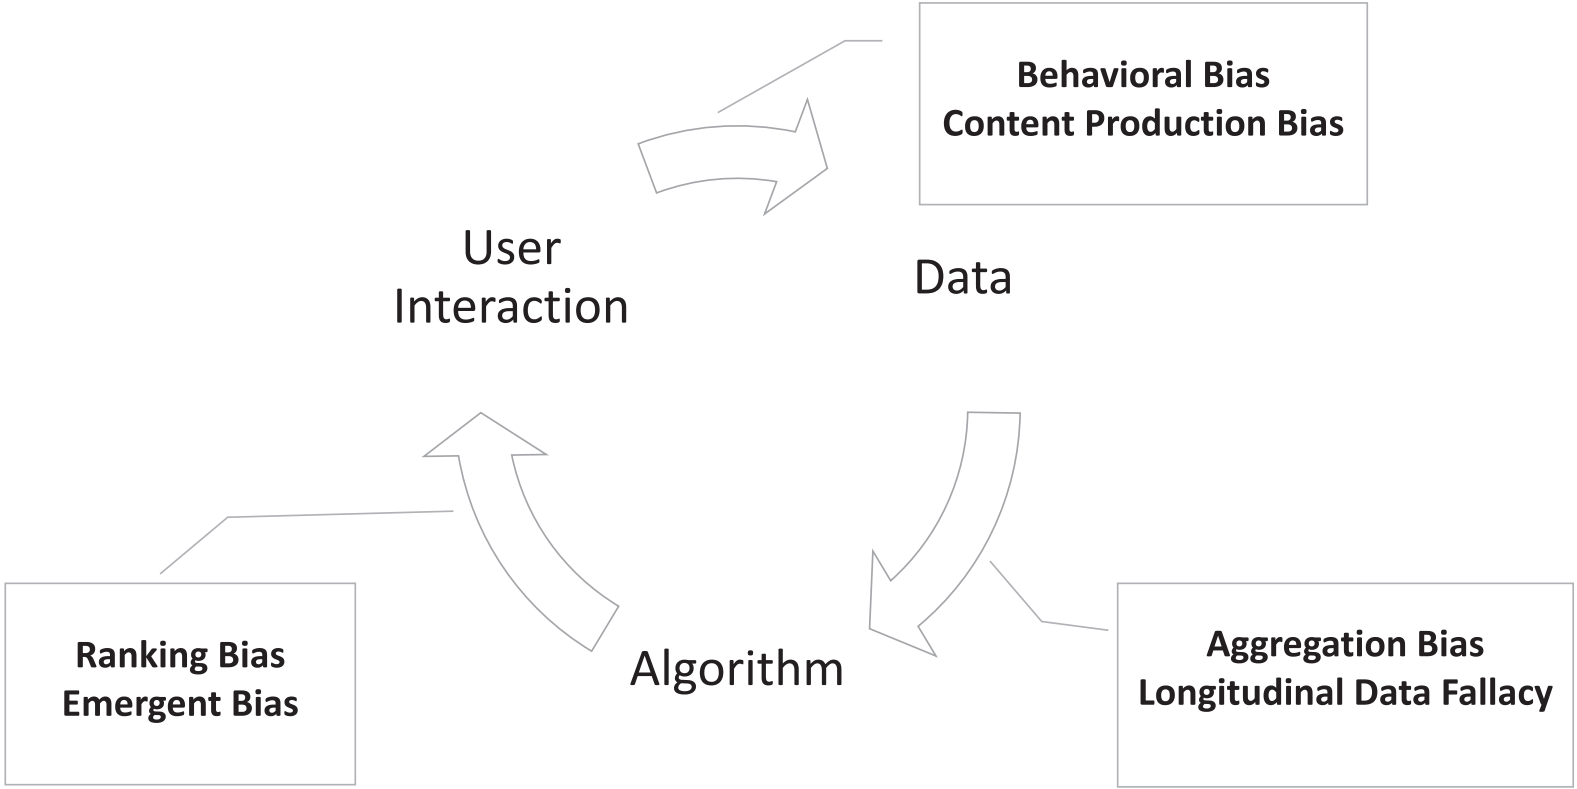
\includegraphics[width=0.8\textwidth]{figures/BiasCategoriesInMLLifecycle.png}
			\caption{Bias definitions in a \gls{ML} lifecycle \autocite{Mehrabi_2021}.}
			\label{fig:bias_definitions_ML_lifecycle}
		\end{figure}
		
		\rawcitationusedstart
		\begin{itemize}
			\item two potential sources of unfairness in machine learning outcomes - those that arise from biases in the data and those that arise from the algorithms ... we observe that biased algorithmic outcomes might impact user experience, thus generating a feedback loop between data, algorithms and users that can perpetuate and even amplify existing sources of bias \autocite{Mehrabi_2021}.
			\item The loop capturing this feedback between biases in data, algorithms, and user interaction is illustrated in Figure 1. We use this loop to categorize definitions of bias in the section below \autocite{Mehrabi_2021}
		\end{itemize}
		\rawcitationusedend
		
		
		\subsection{Bias Types}
		The \autoref{tab:biases_types} aims to provide an overview over what kind of biases exist according to research. The more detailed categories listed in the table try to capture similar kind of biases. This thesis follows roughly the categorization of \textcite{Mehrabi_2021}. Some biases might acctually fit in multiple categories. The definition of the categories including examples of specific biases follows.
		
		\todo{check the c citations in the following chapters}
		
		\begin{table}[H]
			\centering
			\begin{threeparttable}
				\begin{tabularx}{\textwidth}{>{\tblWidthDescription}X|>{\tblWidthContext}X|>{\tblWidthContext}X}
					\toprule
					\textbf{Bias} & \multicolumn{2}{c}{\textbf{Mentioned in Context of}} \\
					& \textbf{\gls{ML}} & \textbf{Dermatology} \\
					%	\midrule
					\multicolumn{3}{l}{\bolditalic{Data Biases}} \\ 
					
					Sampling Biases & X\tnote{1,2,3} & X\tnote{4} \\
					Representation Biases & X\tnote{1} & X\tnote{5,6} \\
					Measurement Biases & X\tnote{1,3} & X\tnote{4,6} \\
					Research Biases & X\tnote{7} & X\tnote{4} \\
					Feature Representation Biases & X\tnote{1,3} & X\tnote{4} \\
					Imaging Biases & & X\tnote{5} \\
					Medical Biases & X\tnote{8} & X\tnote{4} \\
					Temporal Data Biases & X\tnote{1} & X\tnote{4}\\
					
					%	\midrule
					\multicolumn{3}{l}{\bolditalic{Algorithmic Biases}} \\ 
					User-Algorithm Interaction Biases & X\tnote{1} & \\
					External Influence Biases & X\tnote{1} & X\tnote{4} \\
					
					%	\midrule
					\multicolumn{3}{l}{\bolditalic{User Biases}} \\
					Cognitive Biases & X\tnote{1,7} & X\tnote{4} \\
					Behavioral Biases & X\tnote{1,3} & X\tnote{4,5} \\
					Publication Biases &  & X\tnote{4} \\
					Medical Biases & X\tnote{} & X\tnote{4} \\
					
					\bottomrule
				\end{tabularx}
				\begin{tablenotes}
					\footnotesize
					\begin{minipage}{0.33\textwidth}\raggedright
						\item[1] \autocite{Mehrabi_2021}
						\item[2] \autocite{HP_2022}
						\item[3] \autocites{Mester_2022}
					\end{minipage}%
					\begin{minipage}{0.33\textwidth}\raggedright
						\item[4] \autocite{Chakraborty_2024}
						\item[5] \autocite{Young_2020}
						\item[6] \autocite{Montoya_2025}
					\end{minipage}%
					\begin{minipage}{0.33\textwidth}\raggedright
						\item[7] \autocites{Mester_2017}
						\item[8] \autocite{Delgado-Rodriguez_2004}
					\end{minipage}%
				\end{tablenotes}
			\end{threeparttable}
			\caption{Bias categories - grouped according the \gls{ML} lifecycle of \textcite{Mehrabi_2021}}
			\label{tab:biases_types}
		\end{table}
		
		\todo{Feedback Astrid: zu viele Unterkapitel -> anders strukturieren}
		\subsubsection{Data Biases}
		
		\paragraph{Sampling Biases}
		When gathering data, it's usually not possible to gather the data of a whole population. Instead, the data is gathered by sampling. A sample is a subgroup of individuals from the population. To get unbiased results, this sampling process should represent the true population, with a low sampling error \autocites{HP_2022}. This is often achieved with randomized samples. With non-random sampling processes, sampling bias arises. The consequence is, that the insights of one sampled population may not generalize with insights on another sampled popluation \autocite{Mehrabi_2021}.
		
		Those biases can be introduced with a flawed sampling process:
		\begin{itemize}
			\item \textbf{Sampling bias}, due to nonrandom sampling of subgroups, leading to poor generalization \autocite{Mehrabi_2021}
			\item \textbf{Selection bias}, working only on specific subset of the population which is not representative \autocites{Mester_2022}{Chakraborty_2024}
			\item \textbf{Systematic selection bias}, chosen samples differ dramatically from the representative populations; e.g. in dermatology, when only the most severe patient data gets included \autocite{Chakraborty_2024, c5,c6,c33}
			\item \textbf{Ascertainment bias}, tendency to exclude segments from the population due to e.g. cultural differences, such as which patient segment goes to government clinics vs. private clinics (usually influenced by socioeconomic status) \autocite{Chakraborty_2024, c5}
			\item \textbf{Availability bias}, focus on widely available data instead of most representative data \autocites{Chakraborty_2024, c9, c10}{}
			\item \textbf{Survivorship bias}, focus only on pre-selected data, ignoring the initial data-points which got filtered out \autocite{Mester_2022}.
		\end{itemize}
		
		
		\subparagraph{Potential Biases in PASSION}
		PASSION tries to reduce sampling bias in dermatology against high pigmented skin.
		PASSION might introduce (systematic) selection bias or Ascertainment bias, if in the dermatology centers only sickest / more severe patients are seen as indicated by \textcite{Chakraborty_2024}
		PASSION inherits availability bias as it is using \gls{FST} scale.
		Survivorship bias could be relevant for PASSION, if dermatology diseases could be lethal. Further, all patients which are not able to go to one of the dermatology centers which were used in PASSION could be considered to left out by survivorship bias.
		
		\rawcitationstart
		used
		\begin{itemize}		
			\rawcitationusedstart
			\item Sampling Bias. Sampling bias is similar to representation bias, and it arises due to nonrandom sampling of subgroups. As a consequence of sampling bias, the trends estimated for one population may not generalize to data collected from a new population. \autocite{Mehrabi_2021}. This is what the PASSION dataset tries to improve
			
			\item Selection bias - wrong sampling method, working on a specific subset of audience; usually by working only with data that is easy to access \autocites{Mester_2022}{Mester_2017} - statistical bias
			\item Selection bias: Since it is not possible to work with large populations, for most dermatological studies, samples are chosen that are said to be representative of the original population. 
			In selection bias, the selected subgroups are not representative of their original population.
			A variation of this is systematic selection bias, where samples chosen differ dramatically from their representative populations.
			Our experience suggests, such selection bias occurs more commonly in studies conducted in regional referral centers where only the sickest or more severe patients are usually seen.
			For example, a study compared the efficacy of thalidomide vs. prednisolone in hospitalised patients of erythema nodosum leprosum. It derived that thalidomide was more efficacious than steroids in erythema nodosum leprosum. Such findings cannot be generalised to all erythema nodosum leprosum since patients admitted to a regional referral center will likely have more severe disease.5,6,33 \autocite{Chakraborty_2024}
			\item  Availability bias: More emphasis is placed on widely available data than scantily available data. A classic example is the use of antihistamines in pregnancy dermatoses, where nearly all standard books recommend first-generation antihistamine chlorpheniramine because more data is available.9 10. \autocite{Chakraborty_2024} - dermatology
			
			\item Survivorship bias \autocites{Mester_2022}{Mester_2017} - statistical bias
			
			
			\item Ascertainment Bias: This bias is commonly encountered in venereology practice. It is defined as a bias due to the tendency of some segments of the target population to get excluded due to cultural and other differences. For example, in most venereology clinics in government setups, studies show that venereal diseases are commoner in lower socioeconomic status. One reason might be that the higher socioeconomic status people tend to go to private practitioners and thereby get excluded from government-run clinics.9,10 Allocation concealment and blinding are good ways to avoid this. 5. \autocite{Chakraborty_2024} - healthcare
			\rawcitationusedend
		\end{itemize}
		
		even more extensive
		\begin{itemize}
			\item Selection bias is again divided into two types endogenous selection bias and exogenous selection bias. The best example of endogenous selection bias in dermatology is the inclusion of non-response. If a trial tests the efficacy of a particular biologic in psoriasis, the response is usually collected from trial participants via postal services. Certain participants will not respond, although they might have substantially improved. Their exclusion will result in significant differences in efficacy evaluation.33
			Exogenous selection bias results when both treatment and outcome result from dependency on an external variable that is not controlled. For example, if sunlight exposure is not controlled, it will influence both the intervention and control groups since psoriasis is a photosensitive (and photoexcerbated) dermatosis. \autocite{Chakraborty_2024} - dermatology
			
			
			\item survivorship bias - World War II planes \autocite{Silfwer_2017} - https://doctorspin.org/media-psychology/psychology/survivorship-bias/
		\end{itemize}
		
		\rawcitationend
		
		\paragraph{Representation Biases}
		\todo{still describe this category} 
		
		Those biases can be introduced :
		\begin{itemize}
			\item \textbf{Representation bias}, non-representative sample lead to missing subgroups or other representation anomalies, which can be harmful to downstream applications. Popular \gls{ML} datasets suffer from representation bias \autocites{Mehrabi_2021}{M142_Shankar_2017}
			\item \textbf{Population Bias}. Population bias arise when statistics, demographics and characteristics in the sample differ from the target population \autocite{M120_Olteanu_2019}. The data it creates is non-representative for the target population \autocite{Mehrabi_2021}.
			\item \textbf{Aggregation bias} occurs, when "false conclusions are drawn about individuals from observing the entire population". It doesn't matter, whether the subgroups are represented equally in the training set, any generalized assumptions can result in aggregation bias \autocite{Mehrabi_2021}. In medicine, diseases can present themselves differently across genders and ethnicities \autocite{M144_Suresh_2021}. Therefore, diagnostic models need to incorporate those differences to mitigate aggregation bias \autocite{Mehrabi_2021}.
			\item \textbf{Simpson's Paradox} is a type of aggregation bias, which arises in heterogeneous data analysis. Observed associations disappear or reverses in the subgroup data \autocite{Mehrabi_2021}.
		\end{itemize}
		
		
		\subparagraph{Potential Biases in PASSION}
		PASSION tries to mitigate representation bias, by including more FST skin types - however, it could introduce other representation biases
		Aggregation bias and Simpson's Paradox could potentially be an issue when the analyzed skin diseases present themselves differently in patients based on their genetics
		
		
		\rawcitationstart
		used
		\begin{itemize}		
			\rawcitationusedstart
			\item Representation Bias. Representation bias arises from how we sample from a population during data collection process \autocite{M144_Suresh_2021}. Non-representative samples lack the diversity of the population, with missing subgroups and other anomalies \autocite{Mehrabi_2021}.
			\item Popular machine-learning datasets that serve as a base for most of the developed algorithms and tools can also be biased—which can be harmful to the downstream applications that are based on these datasets. ... In \autocite{M142_Shankar_2017}, researchers showed that these datasets suffer from representation bias and advocate for the need to incorporate geographic diversity and inclusion while creating such datasets. \autocite{Mehrabi_2021}
			
			\item Population Bias. Population bias arises when statistics, demographics, representatives, and user characteristics are different in the user population of the platform from the original target population \autocite{M120_Olteanu_2019}. Population bias creates non-representative data. ... More such examples and statistics related to social media use among young adults according to gender, race, ethnicity, and parental educational background can be found in \autocite{M64_Hargittai_2007}. \autocite{Mehrabi_2021}
			
			\item Aggregation Bias. Aggregation bias (or ecological fallacy) arises when false conclusions are drawn about individuals from observing the entire population. An example of this type of bias can be seen in clinical aid tools. Consider diabetes patients who have apparent morbidity differences across ethnicities and genders. Specifically, HbA1c levels, that are widely used to diagnose and monitor diabetes, differ in complex ways across genders and ethnicities. Therefore, a model that ignores individual differences will likely not be well-suited for all ethnic and gender groups in the population \autocite{M144_Suresh_2021}. This is true even when they are represented equally in the training data. Any general assumptions about subgroups within the population can result in aggregation bias. \autocite{Mehrabi_2021}. --> could also be important for dermatology issues!!!
			\begin{itemize}
				\item Simpson’s Paradox. Simpson’s paradox is a type of aggregation bias that arises in the analysis of heterogeneous data [18]. The paradox arises when an association observed in aggregated data disappears or reverses when the same data is disaggregated into its underlying subgroups (Fig. 2(a)). ... After analyzing graduate school admissions data, it seemed like there was bias toward women, a smaller fraction of whom were being admitted to graduate programs compared to their male counterparts. However, when admissions data was separated and analyzed over the departments, women applicants had equality and in some cases even a small advantage over men. The paradox happened as women tended to apply to departments with lower admission rates for both genders. Simpson’s paradox has been observed in a variety of domains, including biology [37], psychology [81], astronomy [109], and computational social science [91].\autocite{Mehrabi_2021}.
			\end{itemize}
		\end{itemize}
		\rawcitationusedend
		\rawcitationend
		
		\paragraph{Measurement Biases}
		How features are chosen, used and measured can lead to biases \autocites{Mehrabi_2021}{M144_Suresh_2021}.
		
		Examples for such biases are:
		\begin{itemize}
			\item \textbf{Measurement bias} in general, e.g. using mismeasured \glspl{proxyVar} lead to misinterpretations of the outcome \autocite{Mehrabi_2021}
			
			\item \textbf{Observer bias} is a subconscious bias which can occur in different forms. Either, researchers projects their own expectations on the research and influence the testers accordingly \autocite{Mester_2022}. In other cases, different observes report the same observation differently \autocite{Chakraborty_2024, c29, c26}
			
			\item \textbf{Annotator bias} is a special form of observer bias. The labeling process of human annotators can be influenced by lots of factors (e.g. personal background, social context) and even minor design choices (e.g. scale order, image context). This can introduce inconsistencies when labeling the data \autocite{Montoya_2025}
			
			\item \textbf{Recall bias}. This bias occurs when queried individuals do not remember things correctly, due to humans selective memory. This can cause misinterpretation, for example when analyzing causes and effects of behaviour on certain diseases in medicine \autocites{Mester_2022}{Chakraborty_2024, c3-6, c2}.
		\end{itemize}
		
		\subparagraph{Potential Biases in PASSION}
		Measurement Bias (proxy var) - Country of Origin in PASSION depending on the interpretation - should not be used for ethnicity, as this is not linked directly to the genes, see example https://medium.com/bcggamma/practice-ai-responsibly-with-proxy-variable-detection-42c2156ad986
		
		Annotator bias regarding skin tone labeling has been investigated in \autocite{Montoya_2025}. PASSION should evaluate its process.
		
		
		\rawcitationstart
		used
		\begin{itemize}		
			\rawcitationusedstart
			\item Measurement Bias. Measurement, or reporting, bias arises from how we choose, utilize, and measure particular features \autocite{M144_Suresh_2021} (e.g. mismeasured proxy variables) \autocite{Mehrabi_2021}. (= e.g. someone who lives at that postal code probably has this ethnicity ); --> could that be an issue with the country of origin feature?
			
			\item This study found that while using skin tone instead of race for fairness evaluations in computer vision seems objective, the annotation process remains biased by human annotators. Untested scales, unclear procedures, and a lack of awareness about annotator backgrounds and social context significantly influence skin tone labeling. This study exposes how even minor design choices in the annotation process, like scale order (dark to light instead of light to dark) or image context (face or no face, skin lesion presence), can sway agreement and introduce uncertainty in skin tone assessments. ... The researchers emphasize the need for greater transparency, standardized procedures, and careful consideration of annotator biases to mitigate these challenges and ensure fairer and more robust evaluations in computer vision. \autocite{Montoya_2025} - demographic dermatology bias
			
			\item Observer bias - projecting expectations onto the research \autocites{Mester_2022}{Mester_2017} - statistical bias
			\item  Observer bias: When different observers view the same observation, they report it differently e.g., different observers may give differing descriptions about subtle features in the histopathology report of a skin biopsy.29 26. \autocite{Chakraborty_2024} - dermatology
			
			\item Recall bias - respondent doesn't remember things correctly; Recall bias is another common error of interview/survey situations. It happens when the respondent doesn’t remember things correctly. It’s not about bad or good memory – humans have selective memory by default. After a few years (or even a few days), certain things stay and others fade. It’s normal, but it makes research much more difficult. \todo{keep an eye on this when recalling evidences!!}
			\autocites{Mester_2022}{Mester_2017} - statistical bias
			\item Memory or recall bias: This is a type of bias where sufferers of a disease, often termed cases, have a greater tendency to recall a particular habit than non-sufferers, viz controls. This results in an uneven distribution of risk factors between the cases and controls. An example of this would be a case-control study to evaluate the association between dental amalgam use and the development of oral lichen planus. Those with lichen planus are more likely to recall a history of dental amalgam use than those who do not have the disease. This difference in recall between a diseased cohort and control has resulted in difficulties in assessing the association between diet and many dermatological diseases – like milk and chocolate consumption and acne, fatty meals and psoriasis, sugary meals and psoriasis, agricultural exposure to insecticides and pemphigus and so on.3–6 2. \autocite{Chakraborty_2024} - dermatology
			
			\rawcitationusedend
		\end{itemize}
		\rawcitationend
		
		\paragraph{Research Biases}
		\todo{consider to move at beginning / out of data biases}
		Researchers and their processes can also be biased in multiple ways:
		\begin{itemize}
			\item \textbf{Funding / Sponsorship bias}, when a study is deliberately supporting those findings, which the sponsor expects \autocites{Chakraborty_2024, c22}{Mester_2017}
			
			\item \textbf{Data dredging bias}. The statistical methods and model are chosen to provide a certain p-value, to improve the probability of the research hypothesis being true. \todo{consider to move this to an own reporting section} \autocite{Chakraborty_2024}
			
			\item \textbf{Hypothetical bias}. Hypothetical questions lead to responses that do not reflect, what interviewees would do in real life. \autocite{Chakraborty_2024, c31, c28} \todo{isn't this a user bias instead?}
		\end{itemize}
		
		\subparagraph{Potential Biases in PASSION}
		Since the PASSION dataset is already published, the research biases might already be introduced. It is not feasible during the duration of this thesis to make an evaluation on those biases. Instead, I would recommend the PASSION team and researcher in general, to check the list above carefully and take measures against them. Maybe, an external evaluation could help to detect and prevent those biases even better.
		
		
		
		\rawcitationstart
		used
		\begin{itemize}		
			\rawcitationusedstart
			\item Funding bias \autocites{Mester_2022}{Mester_2017} - statistical bias
			\item  Industry sponsorship bias: This has now been reclassified as conflict-of-interest bias. In short, the study deliberately supports the findings expected from it by its sponsors. 22.\autocite{Chakraborty_2024} - dermatology
			
			Reporting biases
			\item  Data dredging bias: It is an entirely avoidable bias. This is subdivided into two types – Fishing type and “P-value hacking” type. It involves using multiple statistical methods to get the desired p-value and selecting the statistical model that gives the p-value the author wants. This is “lamentably common” in dermatological research.16 To detect data dredging bias, always perform a “p-curve analysis” while performing a meta-analysis.17,18 Much emphasis is nowadays given to the confidence interval instead of the p-value, which gives an approximate idea of the range in which one can be 95\% (or 90\%, depending on the confidence interval chosen) sure that the result is correct. The confidence interval remains unaffected by p-value dredging. This subject has been reviewed in depth in recent works.18,19 15.\autocite{Chakraborty_2024}
			
			\item Hypothetical bias: Many dermatological researches (and some life quality questionnaires like vitiQoL) use hypothetical questions – like “What would you do when some stranger asks you about your lesion?”. The responses to these questions by the study participants often do not tally with what they would do in real life. This is called hypothetical bias and is avoided by adopting the ex-ante approach.31 28. \autocite{Chakraborty_2024} - dermatology
			\rawcitationusedend
		\end{itemize}
		\rawcitationend
		
		\paragraph{Feature Representation Biases}
		
		Some of those biases are:
		\begin{itemize}
			\item \textbf{Omitted Variable Bias} arises when variables are not included in the model, which leads to situations for which the model is not ready for \autocites{Mehrabi_2021}{Mester_2022}\autocites{M38_Clarke_2005}{M131_Riegg_2008}\autocite{M114_Mustard_2003}.
			\item \textbf{Collider Bias} Two variables can influence a common third variable, the collider variable. When sampling is restricted by this collider variable, it could lead to a distortion  \autocite{Chakraborty_2024, c4,c8,c9}.
		\end{itemize}
		
		
		\subparagraph{Potential Biases in PASSION}
		The ethnicity is omitted in the PASSION dataset which could lead to issues
		See the medical section for more specific collider bias, maybe there could be others
		
		\rawcitationstart
		used
		\begin{itemize}
			\rawcitationusedstart
			\item Omitted Variable Bias. Omitted variable bias4 occurs when one or more important variables are left out of the model \autocites{M38_Clarke_2005}{M131_Riegg_2008}\autocite{M114_Mustard_2003}. Something that the model was not ready for\autocite{Mehrabi_2021}. did not take into account \autocite{Mehrabi_2021}
			\item Omitted variable bias \autocites{Mester_2022}{Mester_2017} - statistical bias
			\item Collider Bias: This is an under-appreciated bias, and often confused with a confounder. This is especially seen in observational studies where it is defined as a distortion produced by the restriction of sampling by a collider variable. A collider variable is defined as one that has an independent effect on the outcome studied apart from the studied variable. In simpler terms, collider bias occurs when exposure and development influence a common third variable. That variable or collider is controlled by study design or in the analysis. An example is the observation that psoriasis patients tend to have more depression and anxiety disorders. Since severe psoriasis patients tend to get hospitalised and also get screened for mental health issues, a spurious association between them could have been obtained due to collider bias. The two variables viz psoriasis and depression converged, i.e., collided, into a single outcome – hospitalization.8,9 4. \autocite{Chakraborty_2024} - dermatology
			\rawcitationusedend
		\end{itemize}
		\rawcitationend
		
		
		\paragraph{Imaging Biases}
		Dealing with images can lead to a whole other set of challenges, which can lead to biases. The challenges are for example technical variations in hardware and software but also differences in how images are gathered or what is in it \autocite{Young_2020}.
		
		Those biases can be introduced :
		\begin{itemize}
			\item \textbf{Image Quality Bias}. The quality of an image (zoom level, focus, lightning) could be associated with the classification \autocite{Young_2020}
			\item \textbf{Visual Artifact Bias}. Other artifacts, such as presence of hair or surgical ink markings on dermatology images, can decrease classification performance \autocite{Winkler et al., 2019 & Bisla et al., 2019 (from Young_2020)}
			\item \textbf{Field of View Bias}. What view is captured in the image can interfere with prediction quality  what is it, consequence \autocite{Mishra et al., 2019 from Young_2020}
		\end{itemize}
		
		
		\subparagraph{Potential Biases in PASSION}
		The PASSION model could learn to associate unrelated visual effects, hair, body parts or image quality with a disease.
		
		
		\rawcitationstart
		used
		\begin{itemize}		
			\rawcitationusedstart
			\item Image quality. Several barriers to \gls{AI} implementation in the clinic need to be overcome with regards to imaging (Figure 1). These include technical variations (e.g., camera hardware and software) and differences in image acquisition and quality (e.g., zoom level, focus, lighting, and presence of hair). For example, the presence of surgical ink markings is associated with decreased specificity (Winkler et al., 2019), field of view can significantly affect prediction quality (Mishra et al., 2019), and classification performance improves when hair and rulers are removed (Bisla et al., 2019). We have developed a method to measure how model predictions might be biased by the presence of a visual artifact (e.g., ink) and proposed methods to reduce such biases (Pfau et al., 2019). Poor quality images are often excluded from studies, but the problem of what makes an image adequate is not well studied. Ideally, models need to be able to express a level of confidence in a prediction as a function of image quality and appropriately direct a user to retake photos if needed. \autocite{Young_2020} - dermatology
			\rawcitationusedend
		\end{itemize}
		\rawcitationend
		
		\paragraph{Medical Biases}
		In \gls{ML} for health care, there are special medical versions of the mentioned biases as well as completely new biases. They require special attention, since they directly influence the diagnosis or treatment of a disease.
		
		Those biases can be introduced:
		\begin{itemize}
			\item \textbf{Berkesonian bias} occurs in hospital-based studies when two variables influence hospital or clinical attendance independently. This can lead to a distorted estimation of the relationship between those variables because the study population of hospitalized patients is not representative of the whole population \autocite{Chakraborty_2024, c3, c7}
			\item \textbf{Informed presence bias}, the probability to get screened for other diseases is higher for people who seek medical care. Like Berkesonian bias, this can lead to misleading interpretations of relationships between two diseases \autocite{Chakraborty_2024, c27, c23}
			\item \textbf{Diagnostic access bias}, depending on the geographical location, individuals have better access to medical care. Therefore, their disease prevalence could appear to be higher and diseases could be diagnosed earlier. \autocite{Chakraborty_2024, c19-c21}
			\item \textbf{Diagnostic reference test bias} is a \textbf{verification bias}, where not all individuals receive the same reference test for the diagnostic process, potentially leading to different diagnoses. \autocite{Chakraborty_2024, c21}
			\item \textbf{Mimicry bias}, exposures to treatment options can cause a disease which presents itself similar to the study disease, which potentially creates misleading data \autocite{Chakraborty_2024, c28, c25}
			\item \textbf{Unacceptable Disease bias}. When a disease is socially unacceptable, it can result in under-reporting of the same disease \autocite{Chakraborty_2024, c30, c27}
			\item \textbf{Healthy volunteer selection bias}, is a type of self-selection bias where the volunteers are in general healthier than the population due to more interest in health \autocite{Delgado-Rodriguez_2004}
		\end{itemize}
		
		\subparagraph{Potential Biases in PASSION}
		Berkesonian bias depending on the chosen hospitals
		Informed presence bias regarding correlation between impedigo and the other diseases
		Diagnostic access bias can somewhat be addressed by PASSION, since its dataset includes samples of later states of diseases. However, in the PASSION context itself, this bias could still be relevant.
		Diagnostic reference test bias could be inherited in the PASSION dataset, depending on how the dermatologists work.
		Mimicry bias is not relevant regarding the exposures since PASSION does not hold any exposure data. However, diseases which mimicry others could lead to issues if they are not detected.
		
		
		
		\rawcitationstart
		used
		\begin{itemize}		
			\rawcitationusedstart
			\item Berkesonian Bias: Named after Dr. Joseph Berkeson, this bias reflects the variation in rates of hospital admission or clinic attendance for different diseases. For example, if a study is conducted to know the effect of pregnancy on syphilis in an antenatal clinic, we are likely to get biased data since the two conditions, viz pregnancy and syphilis, are both likely to affect clinic attendance and all observations related to the relationship between pregnancy and syphilis.7 3. \autocite{Chakraborty_2024} - dermatology
			
			\item  Informed presence bias: Simply, a person attending a health center is more likely to get screened for other unrelated comorbidities than those not attending a health center e.g., the finding psoriasis is associated with depression has now been criticised because those having psoriasis also have a greater chance to be screened for depression since they are already attending a health center.27 23. \autocite{Chakraborty_2024} - dermatology	
			
			\item  Diagnostic Access Bias: Individuals in certain geographical localities have better access to medical care and, hence, may appear to have higher disease prevalence. For example, atopic dermatitis is believed to be commoner in the West – this could be due to better and earlier diagnostic facilities available than in India.19,20 17.\autocite{Chakraborty_2024}
			
			\item  Diagnostic reference test bias: These bias results when all individuals do not receive the same reference test. e.g., direct immunofluorescence studies may not be done for all patients with pemphigus vulgaris some patients may receive only a skin biopsy-based diagnosis. It is a subtype of verification bias. Another variation of this type of bias is partial reference bias, where only some of the study participants receive the index and the reference tests.21\autocite{Chakraborty_2024}
			
			\item  Mimicry bias: When an exposure causes a disease that resembles the study disease, mimicry bias can result. For example, certain drugs are known to cause a pityriasis rosea-like reaction, which, although looks like pityriasis rosea, differs from it.28 25.\autocite{Chakraborty_2024} - dermatology
			
			\item Unacceptable disease bias: This occurs in socially unacceptable diseases like leprosy and STDs, which result in under-reporting.30 27. \autocite{Chakraborty_2024} - dermatology
			
			\item \todo Other such studies were conducted in [\autocite{M54_Fry_2017}] which states that UK Biobank, a large and widely used genetic dataset, may not represent the sampling population. Researchers found evidence of a “healthy volunteer” selection bias. [150] has other examples of studies on existing biases in the data used in the medical domain. [157] also looks at machine-learning algorithms and data utilized in medical fields, and writes about how artificial intelligence in health care has not impacted all patients equally.\autocite{Mehrabi_2021} --> [150] also provides an ovverview over the impact of social determinants on health, such as Economic stability, neighborhood and physical environment, education, food, community and scial context, access to healthcare and quality
			\item The healthy volunteer effect is a particular case: when the participants are healthier than the general population. \autocite{Delgado-Rodriguez_2004}
			\rawcitationusedend
		\end{itemize}
		\rawcitationend
		
		\paragraph{Temporal Biases}
		Differences in populations and their behaviour over time can lead to temporal biases \autocite{M120_Olteanu_2019}.
		Certain studies require to track temporal data, to learn about their behaviour over time. Disease progression is also a factor measured over time \autocite{Mehrabi_2021}. For PASSION, temporal biases are currently irrelevant, since PASSION contains images independently of time and is not tracking the disease progression. Therefore, the listed biases in this chapter are not explained in detail, refer to the sources for further information.
		
		Examples for temporal data biases are:
		\begin{itemize}
			\item \textbf{Longitudinal Data Fallacy} \autocite{Mehrabi_2021}
			\item \textbf{Chronological bias} \autocite{Chakraborty_2024, c9, c13}
			\item \textbf{Immortal time bias} \autocite{Chakraborty_2024, c24, c20}
		\end{itemize}
		
		
		\todo{added until here}
		\subsection{Algorithmic Biases}
		When an algorithm adds biases to unbiased input data one speaks of \textbf{Algorithmic Bias} \autocite{M9_Baeza-Yates_2018}. This could occur due to algorithmic design choices like optimization functions, regularizations and statistically biased estimators \autocite{M44_Danks_2017}.
		
		\rawcitationstart
		used
		\begin{itemize}		
			\rawcitationusedstart
			\item Algorithmic Bias. Algorithmic bias is when the bias is not present in the input data and is added purely by the algorithm \autocite{M9_Baeza-Yates_2018}. The algorithmic design choices, such as use of certain optimization functions, regularizations, choices in applying regression models on the data as a whole or considering subgroups, and the general use of statistically biased estimators in algorithms \autocite{M44_Danks_2017}, can all contribute to biased algorithmic decisions that can bias the outcome of the algorithms.\autocite{Mehrabi_2021}.
			\rawcitationusedend
		\end{itemize}
		\rawcitationend
		
		\paragraph{User Algorithm Interaction Biases}
		\begin{itemize}
			\item \textbf{User Interaction Bias}. This biases can be triggered by the user interface or the user themselves. The user interface influences the user to behave in a certain way, which could introduce bias in the user behaviour. Users impose this (or their own) biased behavior through interaction on the algorithm \autocite{M9_Baeza-Yates_2018}. \textbf{Presentation bias} and \textbf{Ranking bias} are further subtypes mentioned by \textcites{M93_Lerman_2014}{Mehrabi_2021}.
			\item \textbf{Emergent Bias}. When real users interact with an algorithm, this bias arises some time after the design was completed due to changes in population. It appears more likely in user interfaces \autocite{M53_Friedman_1996}.
		\end{itemize}
		
		
		\subparagraph{Potential Biases in PASSION}
		The user interaction biases, especially the emergent bias could potentially become an issue for PASSION, when the project starts to become publicly available \gls{teledermatology}. Also, the interface design should be evaluated, so that no presentation or ranking bias gets introduced.
		
		\rawcitationstart
		used
		\begin{itemize}		
			\rawcitationusedstart
			\item Emergent Bias. Emergent bias occurs as a result of use and interaction with real users. This bias arises as a result of change in population, cultural values, or societal knowledge usually some time after the completion of design \autocite{M53_Friedman_1996}. This type of bias is more likely to be observed in user interfaces, ... This type of bias can itself be divided into more subtypes, as discussed in detail in \autocite{M53_Friedman_1996}. \autocite{Mehrabi_2021}. probably less relevant at the first stage
			
			\item User Interaction Bias. User Interaction bias is a type of bias that can not only be observant on the Web but also get triggered from two sources—the user interface and through the user itself by imposing his/her self-selected biased behavior and interaction \autocite{M9_Baeza-Yates_2018}. This type of bias can be influenced by other types and subtypes, such as presentation and ranking biases. \autocite{Mehrabi_2021}. -- more relevant for later, when the application would become bigger
			\rawcitationusedend
			\begin{itemize}
				\item Presentation Bias. Presentation bias is a result of how information is presented \autocite{M9_Baeza-Yates_2018} (can only click on content they see, could be the case that user does not see all info on web) \autocite{Mehrabi_2021}.
				\item Ranking Bias. The idea that top-ranked results are the most relevant and important will result in attraction of more clicks than others. This bias affects search engines \autocite{M9_Baeza-Yates_2018} and crowdsourcing applications \autocite{M93_Lerman_2014}.\autocite{Mehrabi_2021}.
			\end{itemize}
		\end{itemize}
		\rawcitationend
		
		\paragraph{External Influence Biases}
		
		Those biases can be introduced :
		\begin{itemize}
			\item \textbf{Evaluation Bias}. When inappropriate or disproprtionate benchmarks are used in model evaluation, they can introduce the benchmarks biases into the model. \autocites{M144_Suresh_2021}{M24_Buolamwini_2018}
			
			\item  \textbf{Incorporation bias}. When index tests in diagnostic accuracy studies are part of the reference tests, this results in elevated sensitivity for the index tests \autocites{Chakraborty_2024, c21, c25, c26}{Young_2020}.
			
			\item \textbf{Popularity Bias}. More popular items tend to be exposed more. Popularity metrics can be manipulated though or not reflecting good quality, this can lead to bias \autocites{M117_Ciampaglia_2018}{Mehrabi_2021}.
			
			\item \textbf{Generalization Issues}.  \autocite{} \todo{add those from young}
		\end{itemize}
		
		
		\subparagraph{Potential Biases in PASSION}
		\todo{add}
		
		\rawcitationstart
		used
		\begin{itemize}		
			\rawcitationusedstart
			\item Evaluation Bias. Evaluation bias happens during model evaluation \autocite{M144_Suresh_2021}. This includes the use of inappropriate and disproportionate benchmarks for evaluation of applications such as Adience and IJB-A benchmarks. These benchmarks are used in the evaluation of facial recognition systems that were biased toward skin color and gender \autocite{M24_Buolamwini_2018}, and can serve as examples for this type of bias \autocite{M144_Suresh_2021}. \autocite{Mehrabi_2021}. -- important for this thesis
			
			\item  Incorporation bias: This is principally relevant for diagnostic accuracy studies when the index test forms a part of the reference test, resulting in elevated sensitivity e.g., if one wants to compare the grattage test vs. dermoscopy in psoriasis and does dermoscopy only from areas of grattage positivity, one would get a very high sensitivity for the grattage test because it was incorporated into the reference test, i.e., dermoscopy.25,26 21.\autocite{Chakraborty_2024}
			
			\item Popularity Bias. Items that are more popular tend to be exposed more. However, popularity metrics are subject to manipulation—for example, by fake reviews or social bots \autocite{M117_Ciampaglia_2018}. ... this presentation may not be a result of good quality; instead, it may be due to other biased factors. \autocite{Mehrabi_2021}.
			\rawcitationusedend
		\end{itemize}
		\rawcitationend
		
		
		\subsection{User Biases}
		
		\paragraph{Cognitive Biases}
		Biases which are related to human perception belong to the category of cognitive biases. They are affecting how data should be presented and interpreted \autocite{Mester_2017}
		
		Those biases can be introduced :
		\begin{itemize}
			\item \textbf{Confirmation Bias}. When people have pre-conceptions, they will only listen to the part of presented information which reinforce those "facts", regardless whether the facts are true or not \autocite{Mester_2017}. In health-care, this can be observed when patients report increases in diseases due to potentially nonfactual information they found on the internet \autocite{Chakraborty_2024, c15, c14}.
			\item \textbf{Belief Bias}. A stronger version of the confirmation bias: Someone who is affected by this bias is so sure about their own gut feelings that they will ignore results of a data research project \autocite{Mester_2017}.
			\item \textbf{Previous Opinion Bias}. When performing multiple tests, the knowledge about the outcome of the previous tests probably influences the results \autocite{Chakraborty_2024}
			\item \textbf{Cause-Effect Bias}. The famous senctence "correlation does not imply causation" can be used here - when correlation between two variables is misinterpreted as a cause-effect in the wrong direction, this bias applies  \autocite{Mester_2017}
			\item \textbf{Historical Bias}. Preexisting biases in the world can affect the data generation process \autocite{M144_Suresh_2021}. Even if they reflect the current reality, it is worth to consider whether those biases should affect the algorithms in question \autocite{Mehrabi_2021}.
			\item \textbf{Content Production Bias}. User generated contents can introduce biases by systematical differences in the production process, stucture and appearance, which might stem from the users background \autocite{M120_Olteanu_2019}.
		\end{itemize}
		
		\subparagraph{Potential Biases in PASSION}
		For PASSION, confirmation bias could lead to issues in the initial diagnosis and could therefore lead to biased data labeling. Same with the previous opinion bias. The later can be reduced when it is ensured, that the labeling experts are diagnosing the diseases independently of each other, so that they do not know the previous opinions.
		Cause-Effect bias is lesser an issue for PASSION, since the causes of the diseases are not analyzed. It could more be an inherit problem, that the algorithm learns wrong causes for diseases, such as appearing hair
		Historical bias can affect PASSIONs process in various ways.
		In PASSION context, Content Production Bias could have an impact on how the images are taken.
		
		
		\rawcitationstart
		used
		\begin{itemize}		
			\rawcitationusedstart
			\item  	
			\item Cognitive bias \autocites{Mester_2017} - statistical bias
			
			\item  Previous opinion bias: In performing a second diagnostic test, if the result of a previous test is known, it is likely to influence the result. An extension of this is the Greenwald’s law of lupus: the Sontheimer amendment – anything and everything that happens to a lupus erythematosus patient is correctly or incorrectly attributed to lupus.32 29. \autocite{Chakraborty_2024} - dermatology
			
			\item  Confirmation bias: This bias occurs when study participants have a preconceived notion of their disease that may not be based on facts. For example, we have observed that in North India many tinea patients report an increase in their disease due to taking meat, fish, and other so-called “hot foods”. They may also present information they have collected from the internet which reinforces their beliefs.15 14.\autocite{Chakraborty_2024} - dermatology
			
			\item Cause-effect bias \autocites{Mester_2022}{Mester_2017} - statistical bias
			
			
			\item Historical Bias. Historical bias is the already existing bias and socio-technical issues in the world and can seep into from the data generation process even given a perfect sampling and feature selection \autocite{M144_Suresh_2021}. ... search results were of course reflecting the reality, but whether or not the search algorithms should reflect this reality is an issue worth considering \autocite{Mehrabi_2021} - maybe relevant
			
			\item Content Production Bias. Content Production bias arises from structural, lexical, semantic, and syntactic differences in the contents generated by users \autocite{M120_Olteanu_2019}. \autocite{Mehrabi_2021} -- could the quality of the pictures been related to this as well?	
			\rawcitationusedend
		\end{itemize}
		\rawcitationend
		
		\paragraph{Behavioral Biases}
		
		Those biases can be introduced :
		\begin{itemize}
			\item \textbf{Behavioral Bias}. User behaviour can differ depending on the platforms, contexts, cultures, or datasets \autocite{M120_Olteanu_2019}.
			\item \textbf{Self-Selection Bias}. This subtype of selection bias occurs when study participants can select themselves. Less proactive people, people with less time or interest will be excluded or underrepresented \autocites{Mester_2022}{Mehrabi_2021}. \textbf{Non-Responder bias} is a subtype, where part of the population is not responding e.g. to fill out a survey or post-study responses queried by postal services \autocite{Chakraborty_2024}. \todo{maybe categorize this in the data biases or the healthy volunteer bias here}
			\item \textbf{Social Bias}. When the actions of others affect our judgment, it is called social bias. For example ratings in juries can be affected by this \autocite{M9_Baeza-Yates_2018}.
		\end{itemize}
		
		
		\subparagraph{Potential Biases in PASSION}
		For PASSION the behavioral biases can affect who is going to the dermatologists for what reasons. Therefore, the approach to use data from different countries may be benefitial, since potentially the cultural differences could differ.
		Self-selection is an issue, since only those patients can be included in the database which go to the hospitals.
		
		
		
		\rawcitationstart
		used
		\begin{itemize}		
			\rawcitationusedstart
			\item Self-Selection Bias. Self-selection bias4 is a subtype of the selection or sampling bias in which subjects of the research select themselves. \autocite{Mehrabi_2021}
			\item Self-selection bias - when you let the subjects of the analyses select themselves, less proactive people will be excluded \todo{could be an issue as well for PASSION, couldn't it? since the doctors probably ask the clients. One way to go is to default should be to provide access to the data. but is it ethical?} \autocites{Mester_2022}{Mester_2017}- statistical bias
			A variation of this is non-responder bias, where non-responders to a questionnaire differ significantly from responders.9 9. \autocite{Chakraborty_2024} - dermatology
			
			\item Social Bias. Social bias happens when others’ actions affect our judgment \autocite{M9_Baeza-Yates_2018}. (case where we want to rate or review an item with a low score, but when influenced by other high ratings, we change our scoring thinking that perhaps we are being too harsh [\autocite{M9_Baeza-Yates_2018}, \autocite{M151_Wang_2014}.) \autocite{Mehrabi_2021}
			
			\item Behavioral Bias. Behavioral bias arises from different user behavior across platforms, contexts, or different datasets \autocite{M120_Olteanu_2019}. \autocite{Mehrabi_2021} maybe, people from different countries go to the dermatologist for different diseases, based on cultural differences?
			\rawcitationusedend
			
		\end{itemize}
		\rawcitationend
		
		\paragraph{Publication Biases}
		
		Those biases can be introduced :
		\begin{itemize}
			\item \textbf{Publication Bias}
			\item \textbf{Hot stuff bias} is a subtype of publication bias, where Journals are less critical about trending topics, which lead to more frequent publishing of those topics. This in turn can lead to flawed meta-analyses regarding those topics  \autocite{Chakraborty_2024, c22, c23, c19}.
			\item \textbf{All is Well Bias}. This bias is a different view on the hot stuff bias. Theories which align with the view of the majority are more likely to be pubhlished than an opposing view \autocite{Chakraborty_2024, c7,c10-12}.
			\item \textbf{Rethoric Bias}. Charismatic writing or when the press is more vocal about findings can lead to greater influence over individuals than other available facts \autocite{Chakraborty_2024}.
			\item \textbf{Novelty Bias}. Newer interventions appear to be better. Over time, this effect decreases \autocite{Chakraborty_2024}.
		\end{itemize}
		
		\subparagraph{Potential Biases in PASSION}
		These biases are relevant for all researchers. They should kept in mind when interpreting, publishing and peer-reviewing papers.
		
		
		
		\rawcitationstart
		used
		\begin{itemize}		
			\rawcitationusedstart
			\item Hot stuff bias: Editors of journals may be less critical about topics that are “fashionable” or currently in vogue and consequently end up publishing them more frequently, resulting in publication bias as well as hot stuff bias. It can result in flawed meta-analyses based on these studies. An example is how cutaneous manifestations of COVID-19 were published. Indian Journal of Dermatology Venereology and Leprosy stood out by choosing not to publish anything and everything related to COVID-19, thus reducing hot stuff bias.22,23 19. \autocite{Chakraborty_2024}
			\item All is well bias: It is a subjective bias where theories supported by the majority tend to get more easily published than the opposing view supported by the minority. For example, ideas on the origin of endemic pemphigus supporting autoimmunity are more likely to be published than theories exploring an infectious trigger. According to some authors, this bias is very difficult to eliminate and is a variant of publication bias.10-12 7.\autocite{Chakraborty_2024} - dermatology
			
			\item Rhetoric bias: A more charismatic piece of writing has a greater influence on the study participants than other available literature. An example is the wider use of sunscreen for polymorphous light eruption over photoprotective strategies like umbrellas, broadbrimmed hats, etc, because the lay press is more vocal about sunscreens.14 11. \autocite{Chakraborty_2024} - dermatology
			
			\item  Novelty bias: The newer an intervention, the better it appears, and with time, its efficacy seems to decrease. When ligelizumab, an IgE antagonist was first discovered, ligelizumab was believed to be better than omalizumab; however, evidence soon pointed to the contrary. 16.\autocite{Chakraborty_2024} - dermatology			
			\rawcitationusedend
		\end{itemize}
		\rawcitationend
		
		
		\paragraph{Medical Biases}
		
		Those biases can be introduced :
		\begin{itemize}
			\item \textbf{Popularity Bias}. In medicine, when more popular diseases (usually well-known or stigmatized ones) get compared with less popular diseases, clinic rates can show a distorted view. The more popular diseases appear to be over-represented over more commoner ones \autocite{Chakraborty_2024, c9, c6}.
			\item \textbf{Apprehension Bias}. Fear related to an upcoming procedure can lead to false evaluations, e.g. when measuring blood pressure \autocite{Chakraborty_2024, c13}.
			\item \textbf{Hawthrone bias}. Subjects might modify their behaviour when they know they are being watched. This bias can be practically utilized by introducing regular follow-ups \autocite{Chakraborty_2024, c8}.
			\item \textbf{Centripetal Bias}. Better reputations affect to which physicians or hospitals patients tend to go to. Famous specialists probably see more cases in regards of their specialty than others \autocite{Chakraborty_2024, c12}.
		\end{itemize}
		
		
		\subparagraph{Potential Biases in PASSION}
		PASSION must be careful in interpreting the metadata. Since the data is from hospitals, they could be biased towards more popular diseases.
		PASSION can potentially use Hawthrone bias to improve the work of the annotators.
		Centripetal bias can also be used when selecting the partners to work with.
		
		
		\rawcitationstart
		used
		\begin{itemize}		
			\rawcitationusedstart
			\item Popularity Bias: This bias arises when a particular disease is more popular (i.e. either more well-known or more stigmatised) among the participants than the disease with which it is compared. For example, if a study compares clinic attendance rates among various dermatological disorders, one would see vitiligo patients are over-represented over melasma. While melasma is commoner in the normal population, vitiligo, due to its popularity because of media publicity and other factors, tends to present earlier.9 6. \autocite{Chakraborty_2024} - dermatology
			
			\item  Apprehension bias: This results from fear and apprehensions related to an impending procedure. The classic example is the false elevation of blood pressure because the person is apprehensive of his or her blood pressure being measured.13 A variant of this is the Hawthorne bias, where subjects modify their behavior, such as regularly taking a prescribed drug or exercising, simply because they know they are being watched, but not due to any apprehensions. Hawthorne bias is practically utilised in many leprosy clinics since regular follow-up has been shown to improve adherence to therapy based on Hawthorne bias. 8. \autocite{Chakraborty_2024} - dermatology
			
			\item Centripetal bias: Patients tend to go to more reputed physicians and hospitals than others. For example, a famous or better-known cosmetologist with a good reputation tends to see more cases than other cosmetologists. 12.\autocite{Chakraborty_2024}  - dermatology
			\rawcitationusedend
		\end{itemize}
		\rawcitationend
			
		
		
		\printbibliography[title=Appendix Bibliography]
	\end{refsection}
%\iftrue
%
\iffalse
\end{document}
\fi
